\chapter{脉搏波时域特征集的构建与处理}
\section{引言}
第三章中介绍了多种描述PPG的时域特征,本章在其基础构建了基于时长、角度、斜率与面积等的PPG多维度时域特征集
同时,也将PPG信号的原始采样值作为特殊的描述特征,构建了PPG采样值时域特征集。本章详细介绍了这两类特征集的处理构建方式,为利用ML相关算法为PE的识别分析这一具体问题做好了数据准备。
另外,本章也明确了利用PPG数据通过ML方法对PE识别这一问题进行研究的具体目标,并按ML模型构建的一般要求,对两个特征集进行了预处理工作。
本章研究内容的框架图如\autoref{fig:frameworks4}所示。

\begin{figure}[htbp]
  \centering
  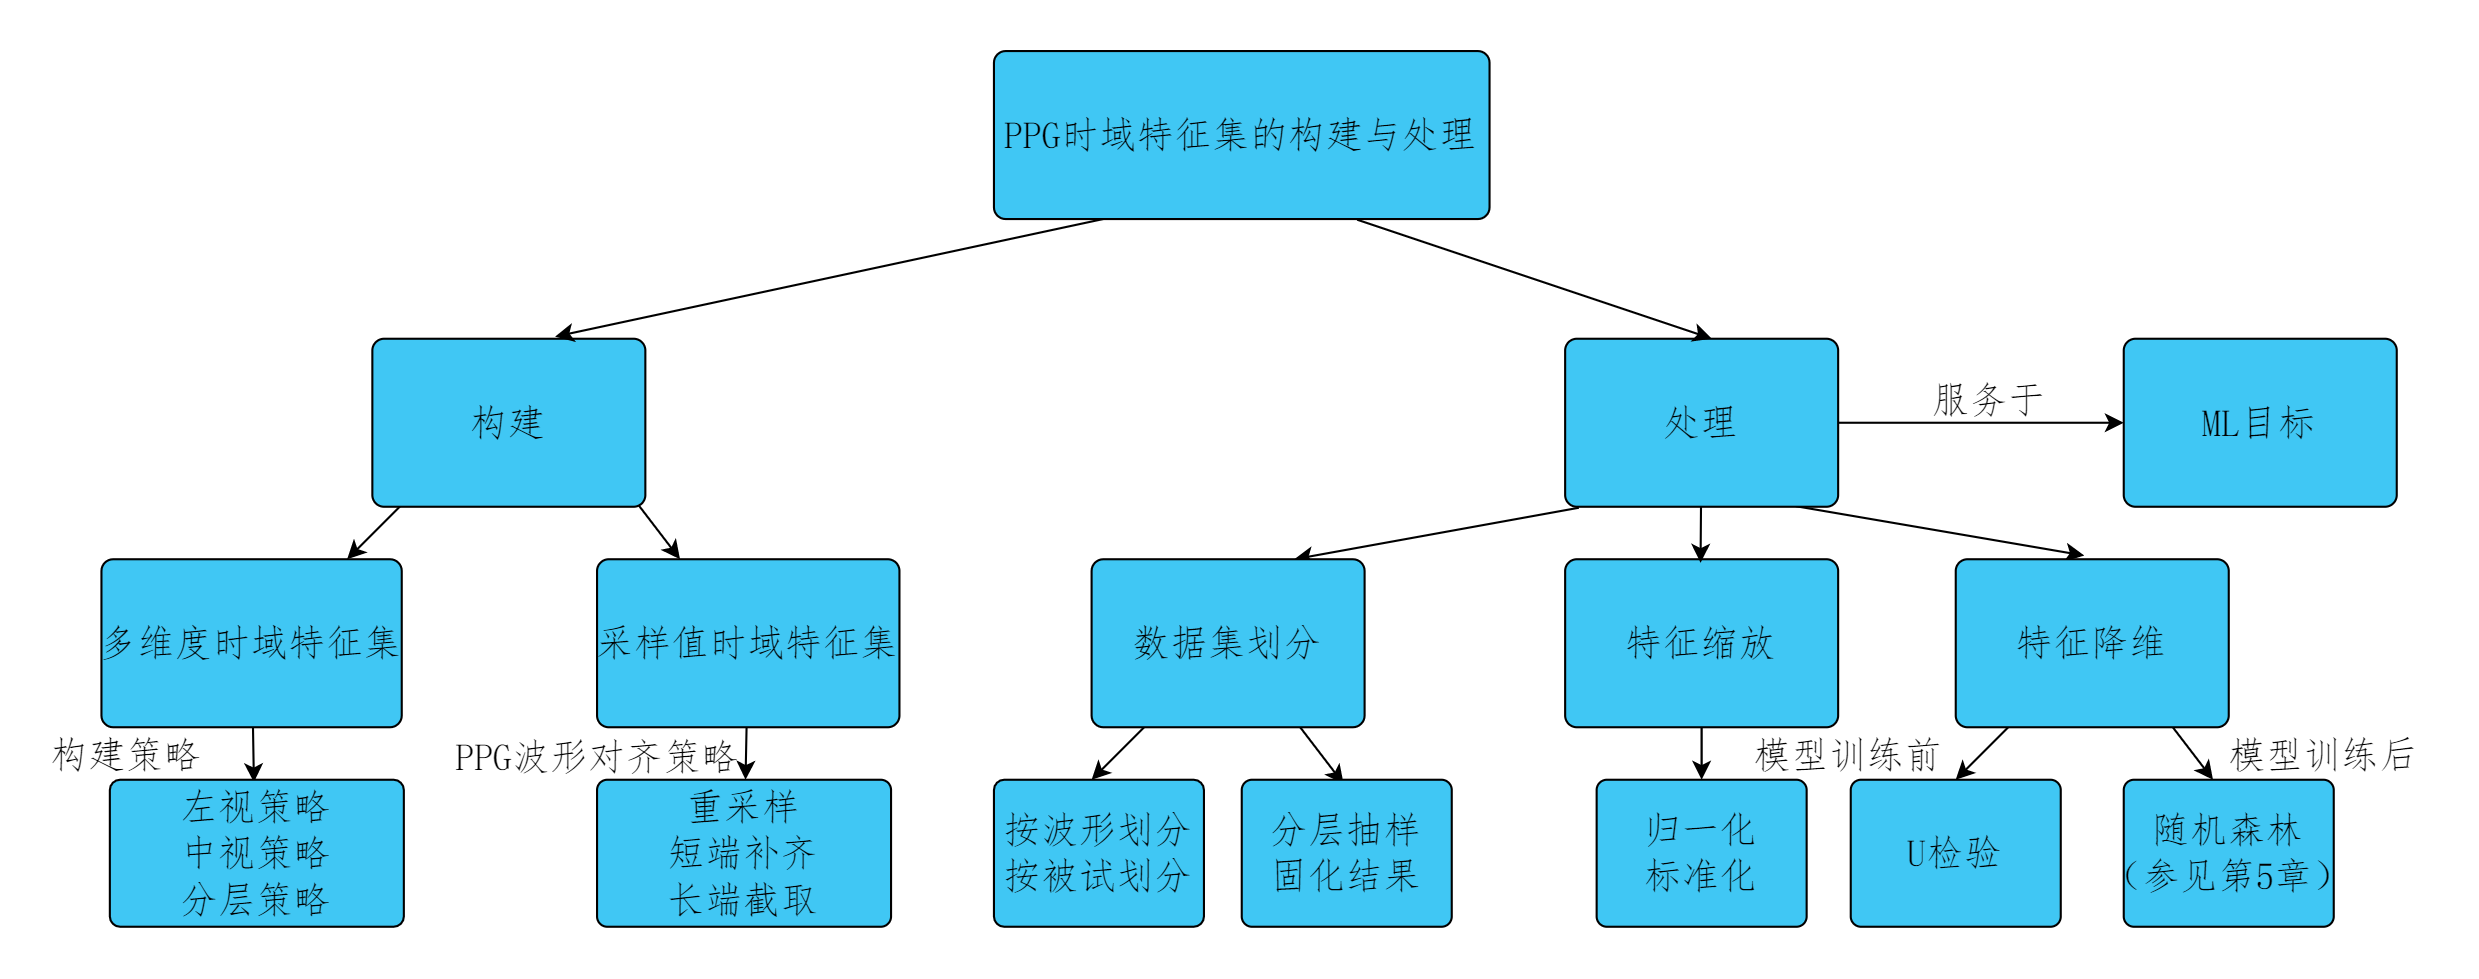
\includegraphics[width=\linewidth]{features/frameworks4}
  \caption{\label{fig:frameworks4}第四章研究内容框架}
\end{figure}
% \vspace{-0.5cm} 


\section{基于波形的新型时域特征参数设计}
在总结前人研究基础上,本研究结合脉搏波形态特点,设计了多种新型时域描述参数,以求从新的角度完成对脉搏波波形特征的描述。

一、波形特征的设计基础

以纯数学的角度来看,PPG的信号波形可以近似描述为从一条往复于水平基线与波峰之间的双向路径。一般而言,由于PPG信号的上升支通常较下降支更为简单,该双向路径可以进一步简化为从波峰下降至水平基线的一条单向路径,只要完成对该单向路径的描述
即可类比完成上升支的描述,从而完成对整个脉搏波波形的描述,如\autoref{fig:road}所示。
\begin{figure}[htbp]
  \centering
  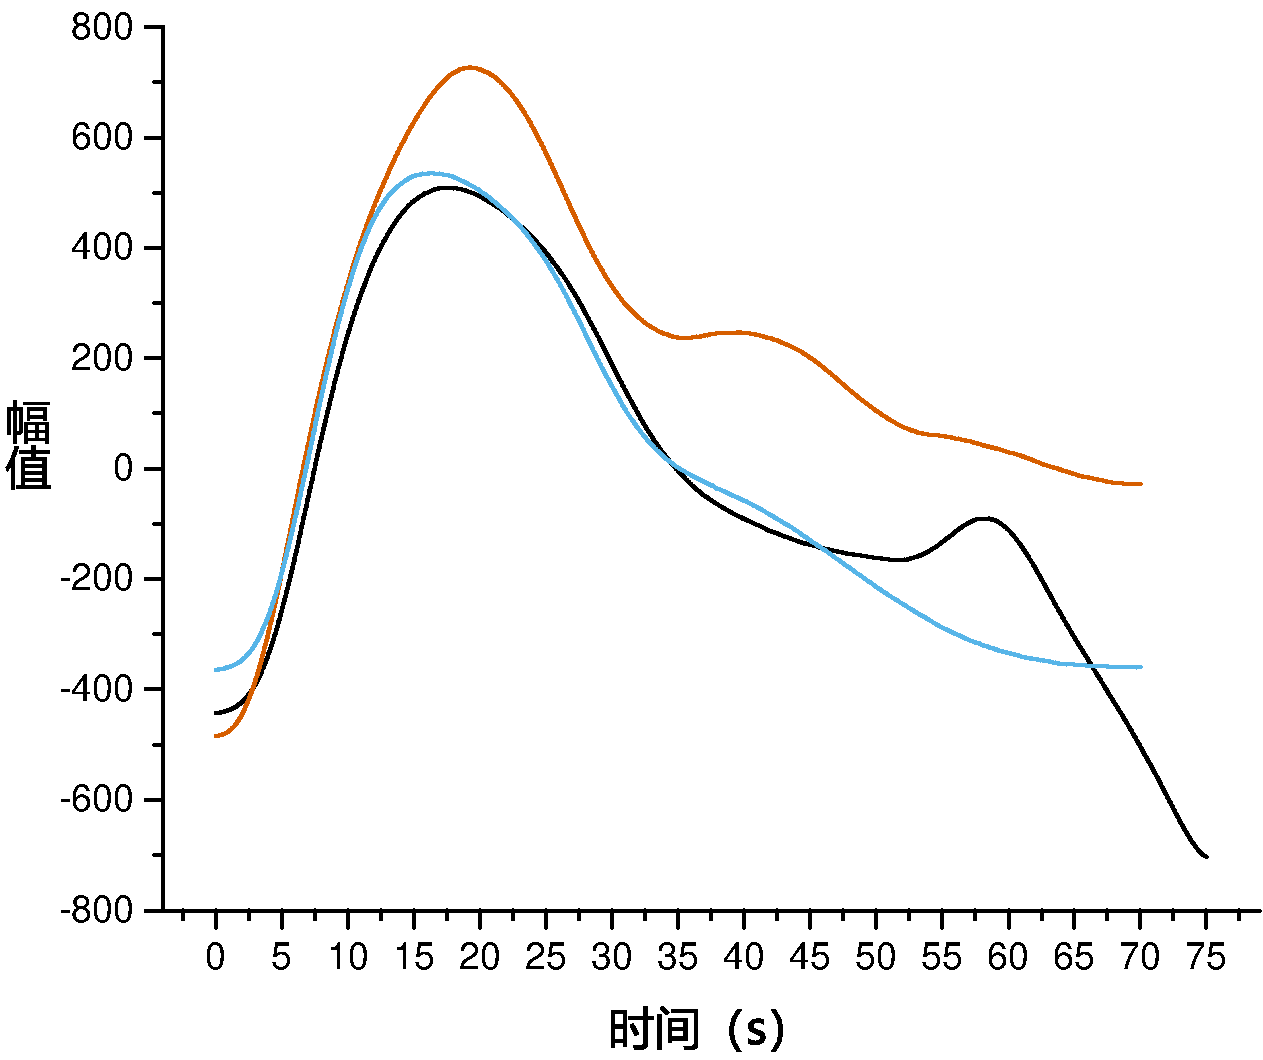
\includegraphics[width=.6\linewidth]{pulse_preprocess/pulsecontrast}
  \caption[同一名被试PPG信号三段波形对比]{\label{fig:pulsecontrast}同一名被试PPG信号三段波形对比。波形按起点时间对齐,此外无任何其他预处理操作。可以看到三段波形在重搏的显著程度、时长、幅值等方面均有所差异。}
\end{figure}

\begin{figure}[htbp]
    \centering
    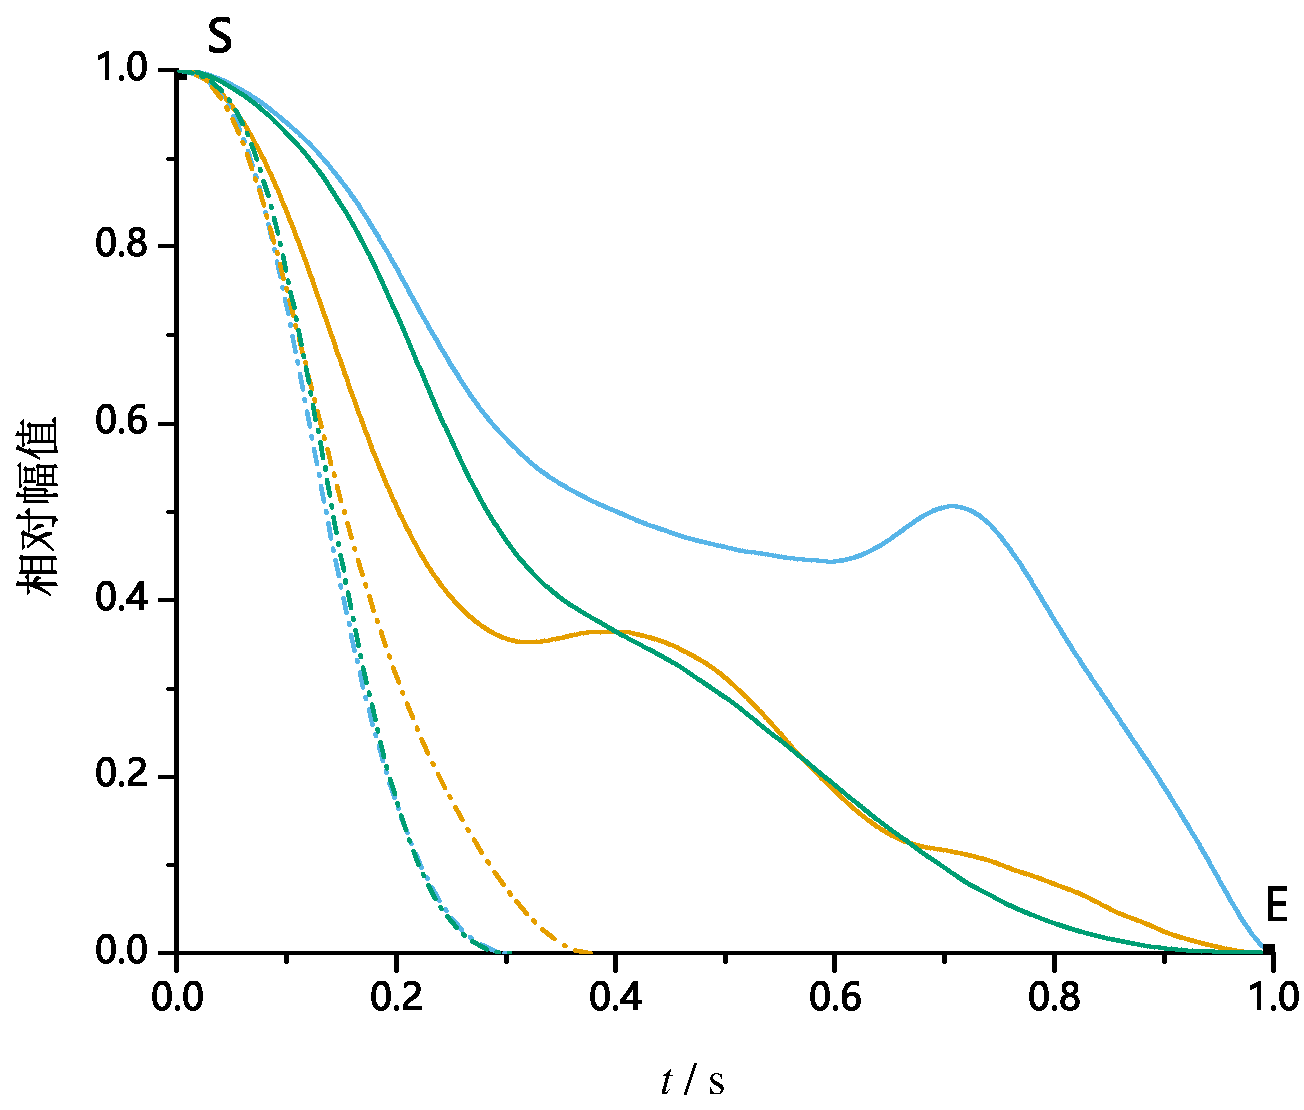
\includegraphics[width=.6\linewidth]{pulse_preprocess/road}
    \caption[脉搏波波形的单向路径表示]{\label{fig:road}脉搏波波形的单向路径表示。其中三条路径由\autoref{fig:pulsecontrast}所示的同一被试的三段波形对应线形变换得来。同一颜色的实线部分与虚线部分对应同一个脉搏波的下降支与上升支
    ,其中,下降支按一定比例缩放至目标区间内,上升支水平反向按同一比例反向进行了缩放。}
\end{figure}

由信号的采样定理可知,对上述路径的描述可通过对路径上一系列点的描述来完成。不失一般性,若将下降支的单向路径的起点坐标与终点坐标分别设置为S$(0,1)$与E$(1,0)$。
对于该路径上任意一点P,可以用原点O坐标$(0,0)$与路径始末点坐标S、E等为基本参照点,以及P
在X轴、Y轴上的投射点$P_x$、$P_y$等衍生参照点进行对该点进行描述,如\autoref{fig:point}所示。
此时对P点进行描述可使用\autoref{tab:pointsdesc}中的定义参数指标,部分参数指标的归一化/类归一化无量纲形式也在表中进行了说明。
% 同一类型下关于起始S、E两点对偶的参数只保留了一个。
\begin{figure}[htbp]
    \centering
    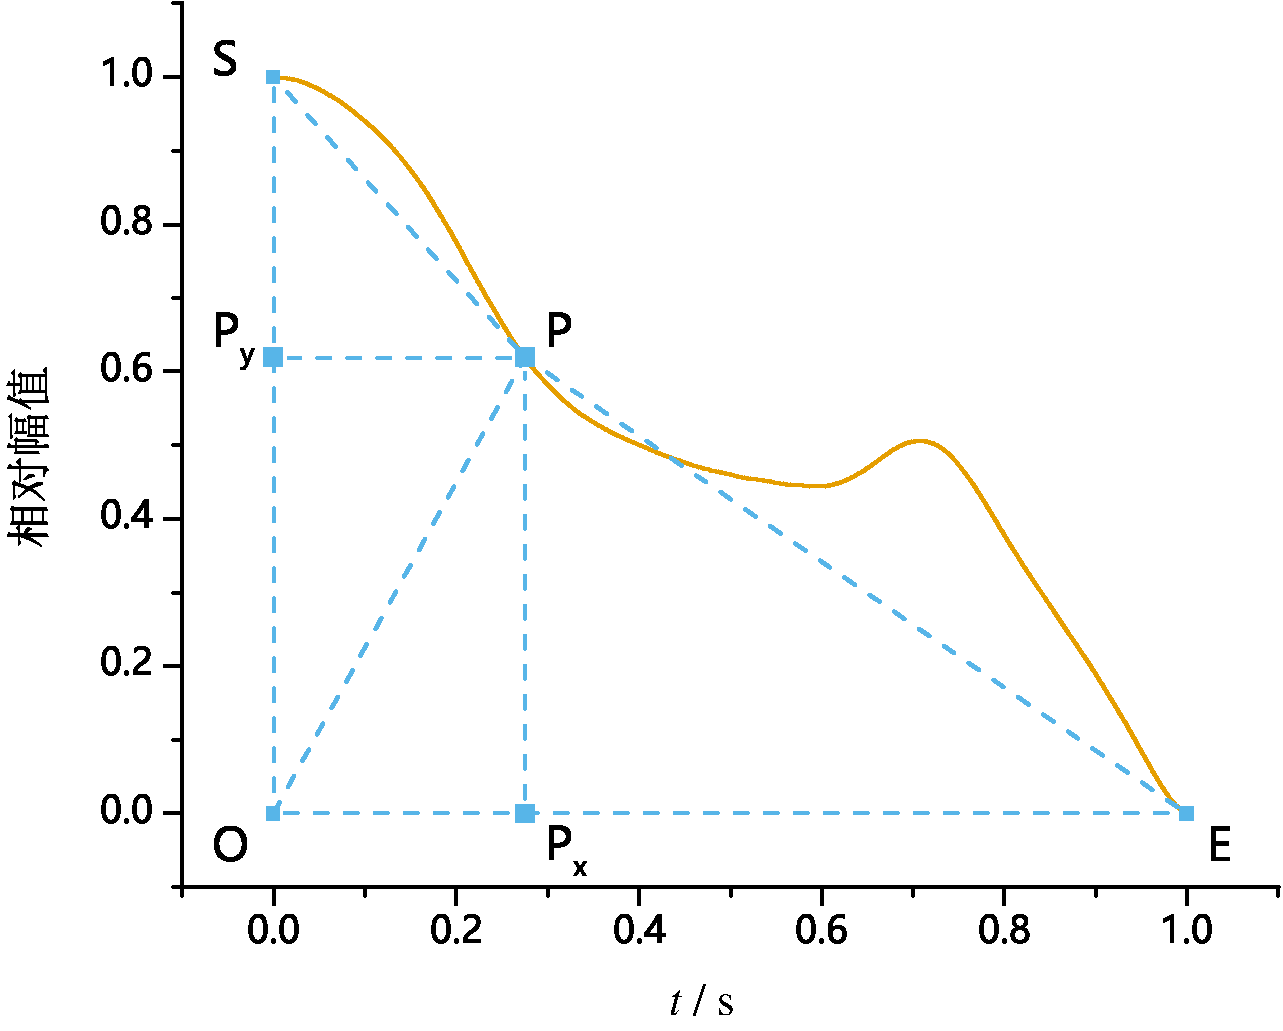
\includegraphics[width=.6\linewidth]{pulse_preprocess/point}
    \caption{\label{fig:point}单向路径上点的描述}
\end{figure}
\begin{center}
    \zihao{-5}
    % Plan A
    % \setlength\LTleft{0pt}
    % \setlength\LTright{0pt}
	% \begin{longtable}{@{\extracolsep{\fill}}|c|c|c|c|c|}
    % Plan B
    % m表示居中,p为置顶,b为置底
    % 列宽总计16cm,各列按需分配长度,p{x-0.43cm}<{\centering}即可
    % \begin{longtable}{p{1.6cm}<{\centering}p{4.1cm}<{\centering}p{2.1cm}<{\centering}p{4.1cm}<{\centering}p{2.1cm}<{\centering}}
    \begin{longtable}{m{1.57cm}<{\centering}m{4.07cm}<{\centering}m{2.07cm}<{\centering}m{4.07cm}<{\centering}m{2.67cm}<{\centering}}
		\caption{单向路径上任意一点的描述指标一览}\\
		\label{tab:pointsdesc}\\
		\topline
        \colorhead  & \multicolumn{2}{c}{\textbf{原始数值表达}} & \multicolumn{2}{c}{\textbf{归一化表达}} \\
        \colorhead \multirow{-2}{*}{\textbf{参数类型}}  & 物理意义 & 表达式或公式 & 物理意义 & 表达式或公式 \\
        \midline
        \endfirsthead
        \caption[]{(续)}\\
        \topline
        \colorhead  & \multicolumn{2}{c}{\textbf{原始数值表达}} & \multicolumn{2}{c}{\textbf{归一化表达}} \\
        \colorhead \multirow{-2}{*}{\textbf{参数类型}}  & 物理意义 & 表达式或公式 & 物理意义 & 表达式或公式 \\
        \midline
        \endhead 
        \midline
        \endfoot
        \bottomline
        \endlastfoot
        \colorrowa                             & Y轴方向下降高度           &   $SP_y$      &  Y轴方向下降比例     & $\frac{SP_y}{OS}$ \\
        \colorrowa                             & P点高度                  &   $OP_y$       &    P点高度与波峰比值   & $\frac{OP_y}{OS}$ \\
        \colorrowa                             & 从S点到P点所用时间        &    $OP_x$   &      起点至P点所用时间与下降支总时长比值 & $\frac{OP_x}{OE}$ \\
        \colorrowa                             & 从P点到E点所用时间        &    $EP_x$   &      P点至终点E所用时间与下降支总时长比值 & $\frac{EP_x}{OE}$ \\
        \colorrowa                             & OP两点间几何距离        &    $OP$   &  OP两点距离与SE两点距离之比     & $\frac{OP}{SE}$ \\
        \colorrowa                             & SP两点间几何距离        &    $SP$   &  SP两点距离与SE两点距离之比     & $\frac{SP}{SE}$ \\
        \colorrowa \multirow{-7}*{线段}         & PE两点间几何距离        &    $PE$   &  PE两点距离与SE两点距离之比     & $\frac{PE}{SE}$ \\
        \colorrowc                             &  SP两点间曲线弧长     &  $L_{\overset{\frown}{SP}}$     &     SP两点间曲线弧长与SE两点直线距离之比  & $\frac{L_{\overset{\frown}{SP}}}{SE}$ \\
        \colorrowa \multirow{-2}*{曲线长度} &  PE两点间曲线弧长   &   $L_{\overset{\frown}{PE}}$    &    PE两点间曲线弧长与SE两点直线距离之比  &  $\frac{L_{\overset{\frown}{PE}}}{SE}$\\
        \colorrowa                             &  线段SP的斜率     &  $-\frac{SP_y}{PP_y}$     &   /    &  /  \\
        \colorrowa                             &  线段PE的斜率     &   $-\frac{P_yP_x}{EP_x}$    &    /  &  /   \\
        \colorrowa \multirow{-3}*{斜率}        &  线段OP的斜率    &    $\frac{PP_y}{PP_x}$   &    /   &  /     \\
        \colorrowc                             &  $\angle SPP_y$的弧度      & $\arctan(\frac{SP_y}{PP_y})$     &    /  &  /   \\
        \colorrowc                             &   $\angle POE$的弧度    &  $\arctan(\frac{P_yP_x}{EP_x})$      &    /  &  /   \\
        \colorrowc \multirow{-3}*{弧度(角度)}&   $\angle PEO$的弧度   &  $\arctan(\frac{PP_y}{PP_x})$         &    /  &  /   \\
        \colorrowa                             &    坐标轴、曲线与$PP_y$以上围成的面积   &  $\int_{P_y}^{S}{P(t)dy} $     &   前述面积与整体面积之比    & $\frac{\int_{P_y}^{S}{P(t)dy}}{\int_O^E{P(t)dx}}$ \\
        \colorrowa                             &   坐标轴、曲线与$OP$以左围成的面积   &    $\int_{O}^{P_x}{P(t)dx}-S_{\triangle OPP_x}$   &  前述面积与整体面积之比     & $\frac{\int_{O}^{P_x}{P(t)dx}-S_{\triangle OPP_x}}{\int_O^E{P(t)dx}}$ \\
        \colorrowa                             &   坐标轴、曲线与$PP_x$以左围成的面积   &   $\int_{O}^{P_x}{P(t)dx}$    &  前述面积与整体面积之比     & $\frac{\int_{O}^{P_x}{P(t)dx}}{\int_O^E{P(t)dx}}$ \\
        \colorrowa \multirow{-4}*{面积}        &    曲线与$SP$围成的面积   &   $\int_{P_y}^{S}{P(t)dy}-S_{\triangle SPP_y} $    &   /    &  /\\
	\end{longtable}
\end{center}

结合\autoref{tab:pointsdesc}与\autoref{fig:point}不难发现,只要在描述路径上任意确定一点$P$,与$P$关联的线段指标、曲线长度指标、斜率指标、弧度指标及面积指标等都可以得到确定并有与之对应的唯一数值。
反之,若以\autoref{tab:pointsdesc}中某一指标为基准,并在该指标的值域内选定一具体数值,则在描述路径上也可以确定与之对应的参考点$P'$,进一步可由$P'$得到其他描述参数的具体数值。
前文介绍的诸多学者的在各项研究中提出的PPG描述参数均不外乎是这样的过程。

二、脉搏波波形特征描述向量

本研究提出的脉搏波特征描述向量(photoplethysmographic feature vector,PPGFV)是对一类量化PPG波形形态特点特征参数的统称。
与前文介绍的诸多仅用一个数值来表征PPG的参数不同,PPFV最显著的特点在于其用一组相互联系的数值来完成对PPG波形的量化描述
\begin{equation}
    \label{equ:featurevector}
    \boldsymbol {V_n}=[v_0,v_1,\cdots,v_{n-1}]
\end{equation}
其中,$n$是特征描述向量的维数,可以视情况人工设定。在本研究中,$n$的取值一般在[8,10]。

若设定原始信号某一PPG波形的采样点数为$N$,则该原始采样数据可以视为$n=N$的特殊PPFV;同理,当该波形经插值处理后的数据可以看成$n>N$的超维PPFV;
最后,使用此前介绍的各类时域参数对波形进行描述时,这些参数可视为$n=1$的特殊PPFV。
显然,在这一过程中可以发现,PPFV对波形的描述能力随着其向量维数的增加而增强,与之相反的,对波形的抽象与概括能力在此过程中则是削弱的。
这一现象可以用信息论中的编码理论进行解释,即通讯过程中在信源原始符号不变的情况下,
增加变换编码的输出符号长度可以提高系统的信息传输能力\cite{Zhao2017}。
从这个角度理解,PPFV是在变换编码背景下一种编码长度与信息描述能力的折中与妥协。

另一方面,PPFV的定义中存在着用来描述的数值需要有相互联系的限制。这里的相互联系可以理解为按照一定的规则在脉搏波上选取$n$个数据点,并从上小节波形特征的设计基础概括的\autoref{tab:pointsdesc}中
选取同一个参数完成n个具体数值的计算,即可得到一个实例化的$n$维向量PPFV。其中的规则是指对这$n$个点的采样方式,可从线段、曲线长度、斜率、弧度及面积等方面均匀或非均匀采样完成。

三、面积类特征参数的优化

重新考察\autoref{fig:areafeature}、\autoref{tab:areafeature}与\autoref{fig:point}、\autoref{tab:pointsdesc}中所示的各种面积类参数可以发现,这类面积类特征的计算过程多数涉及到累加积分运算,会不可避免地导致
PPG波形的细节信息无法在最终的数值中得到体现
\begin{equation}
    \label{equ:area1}
    S = \int_{t_0}^{t_n}P(t)dt \approx \frac{\Delta t}{2} \sum_{i=0}^{n-1}{(P(i)+P(i+1))}
\end{equation}
换言之,我们无法仅从面积类参数的数值上反推其原始波形的细节特征。两个在形态上迥异的PPG波形可能在某一面积类参数上具有相同数值。
为弥补此类面积参数对细节描述的不足,一种最直接的思路是使用\autoref{equ:area1}计算数值时,给予每个累加项一定的权值,即
\begin{equation}
    \label{equ:area2}
    S \approx \frac{\Delta t}{2} \sum_{i=0}^{n-1}{k_{i} (P(i)+P(i+1))}
\end{equation}
其中,加权系数$k_{i}$必须要进行一定的设计,需要能在反映细节的同时也降低权值本身的影响。
\begin{figure}[h]
    \centering
    \subfigure[\label{fig:pow}幂函数簇在0<x<1区间内图像。]{
    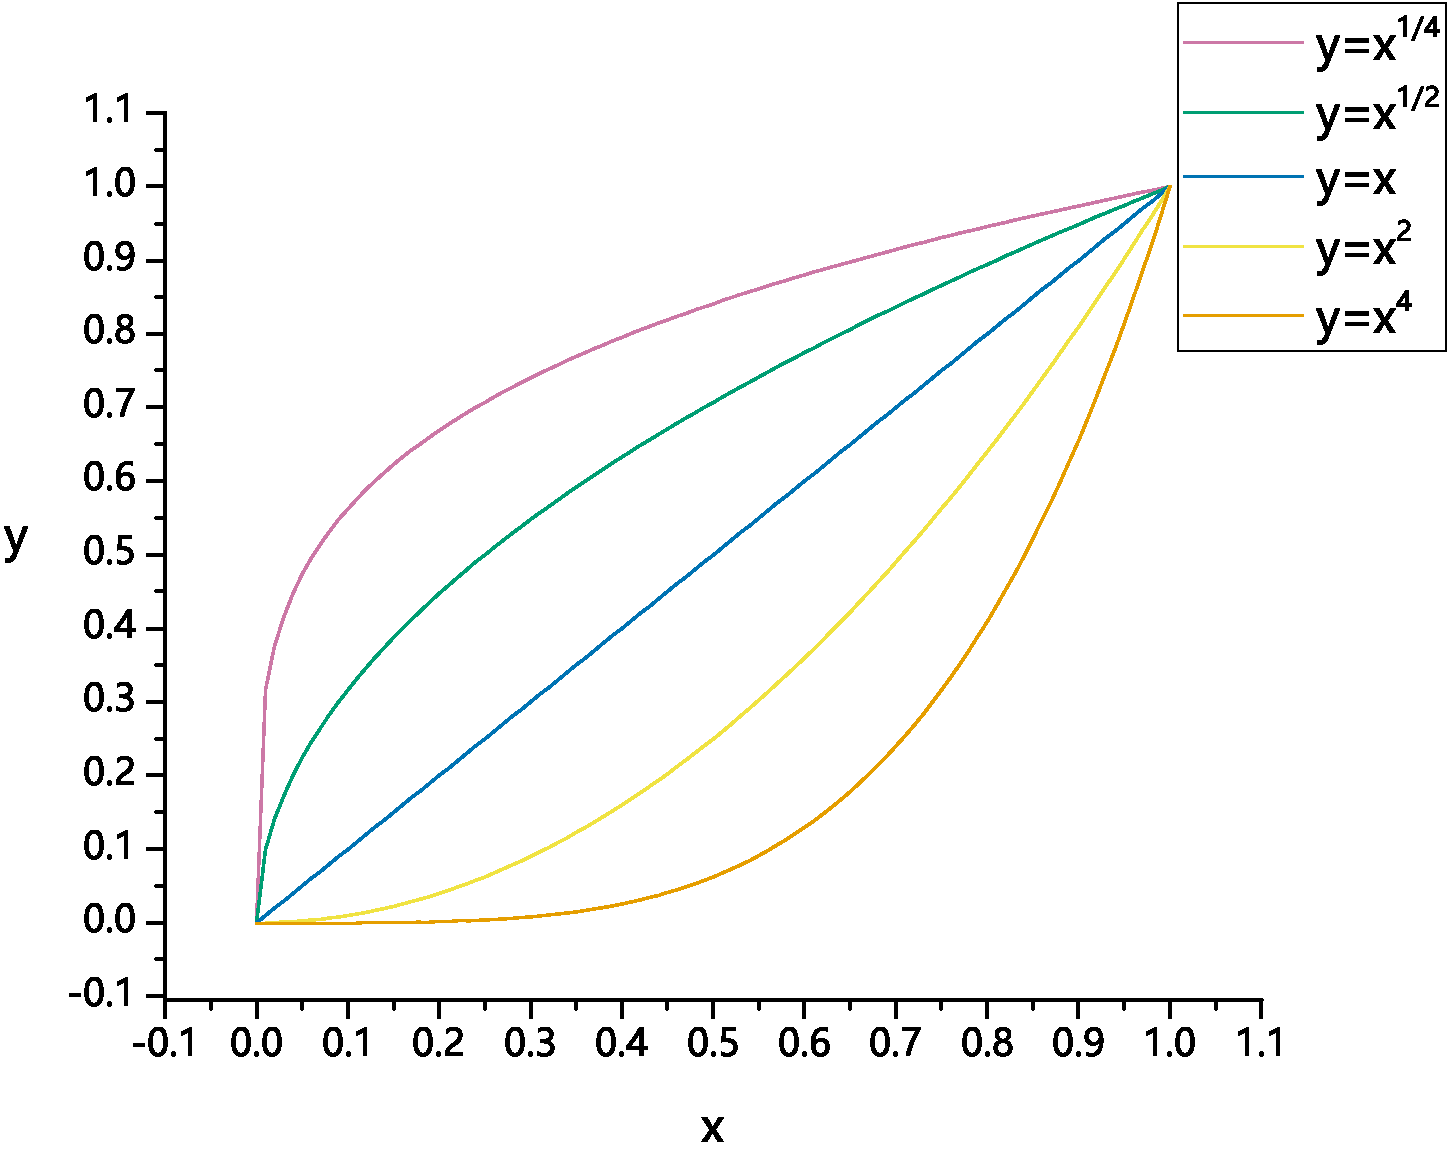
\includegraphics[width=5.5cm]{pulse_preprocess/pow}
    }
    \quad
    \subfigure[\label{fig:edi1}对\autoref{fig:pulsecontrast}中脉搏波波形进行EDI计算 I]{
    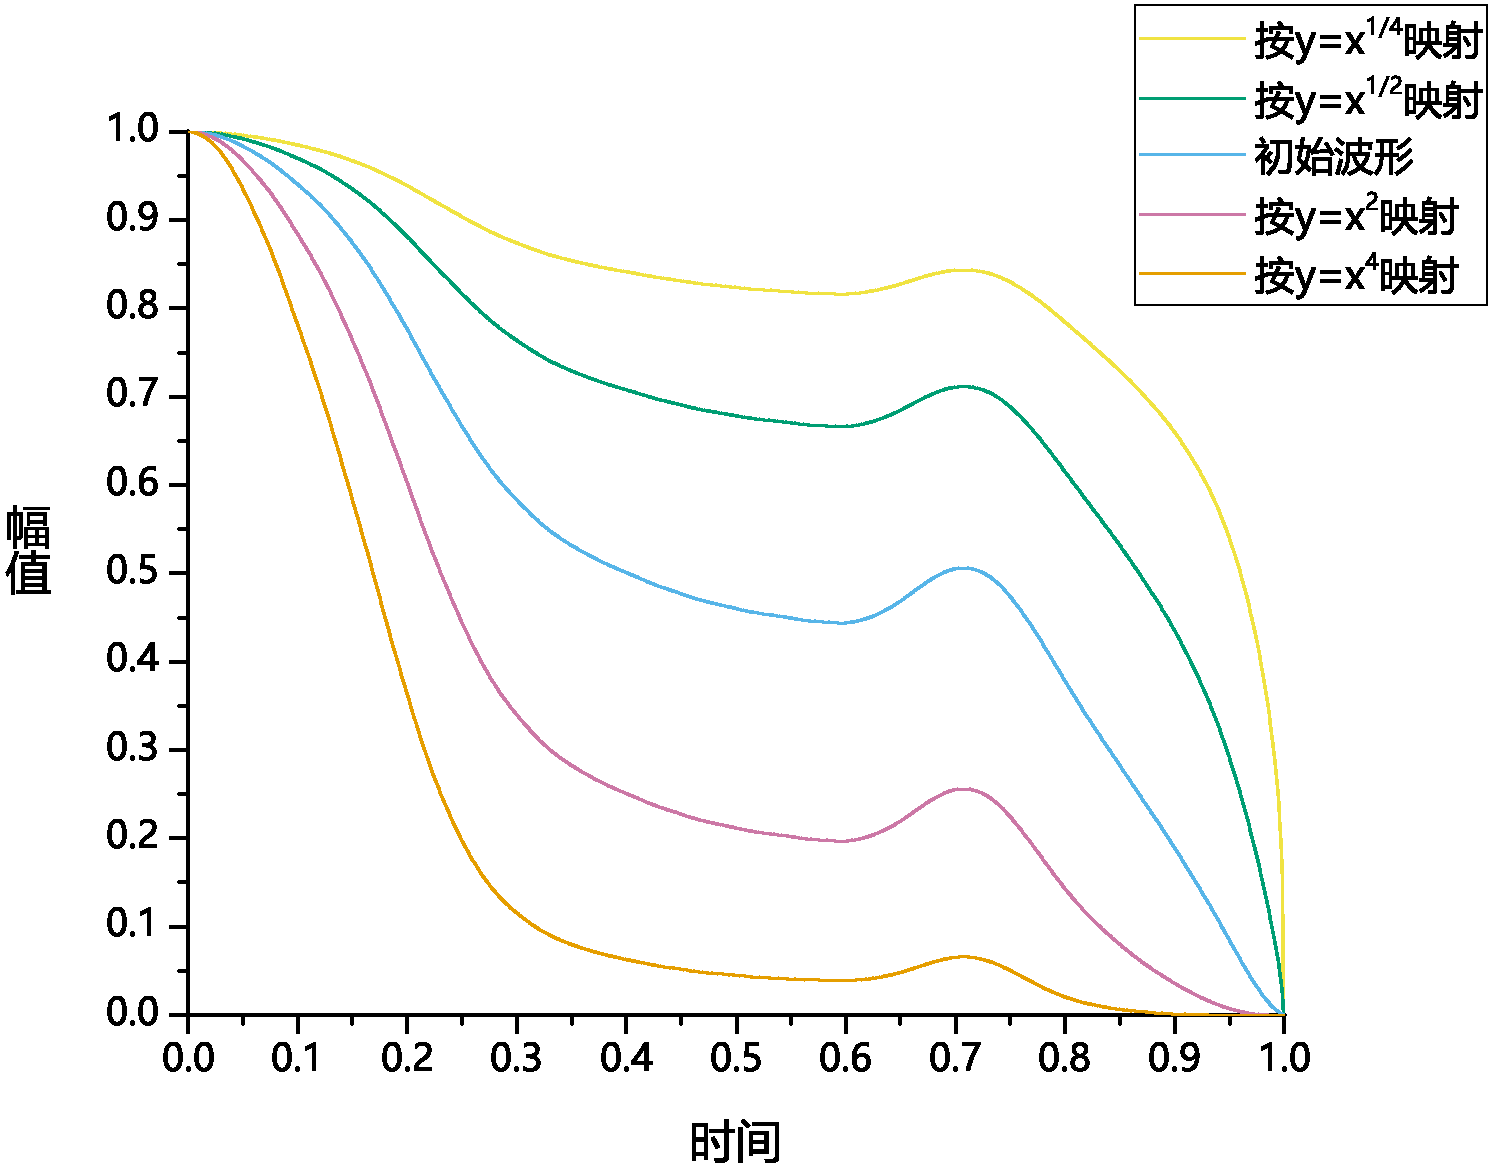
\includegraphics[width=5.5cm]{pulse_preprocess/edi1}
    }
    \quad
    \subfigure[\label{fig:edi2}对\autoref{fig:pulsecontrast}中脉搏波波形进行EDI计算 II]{
    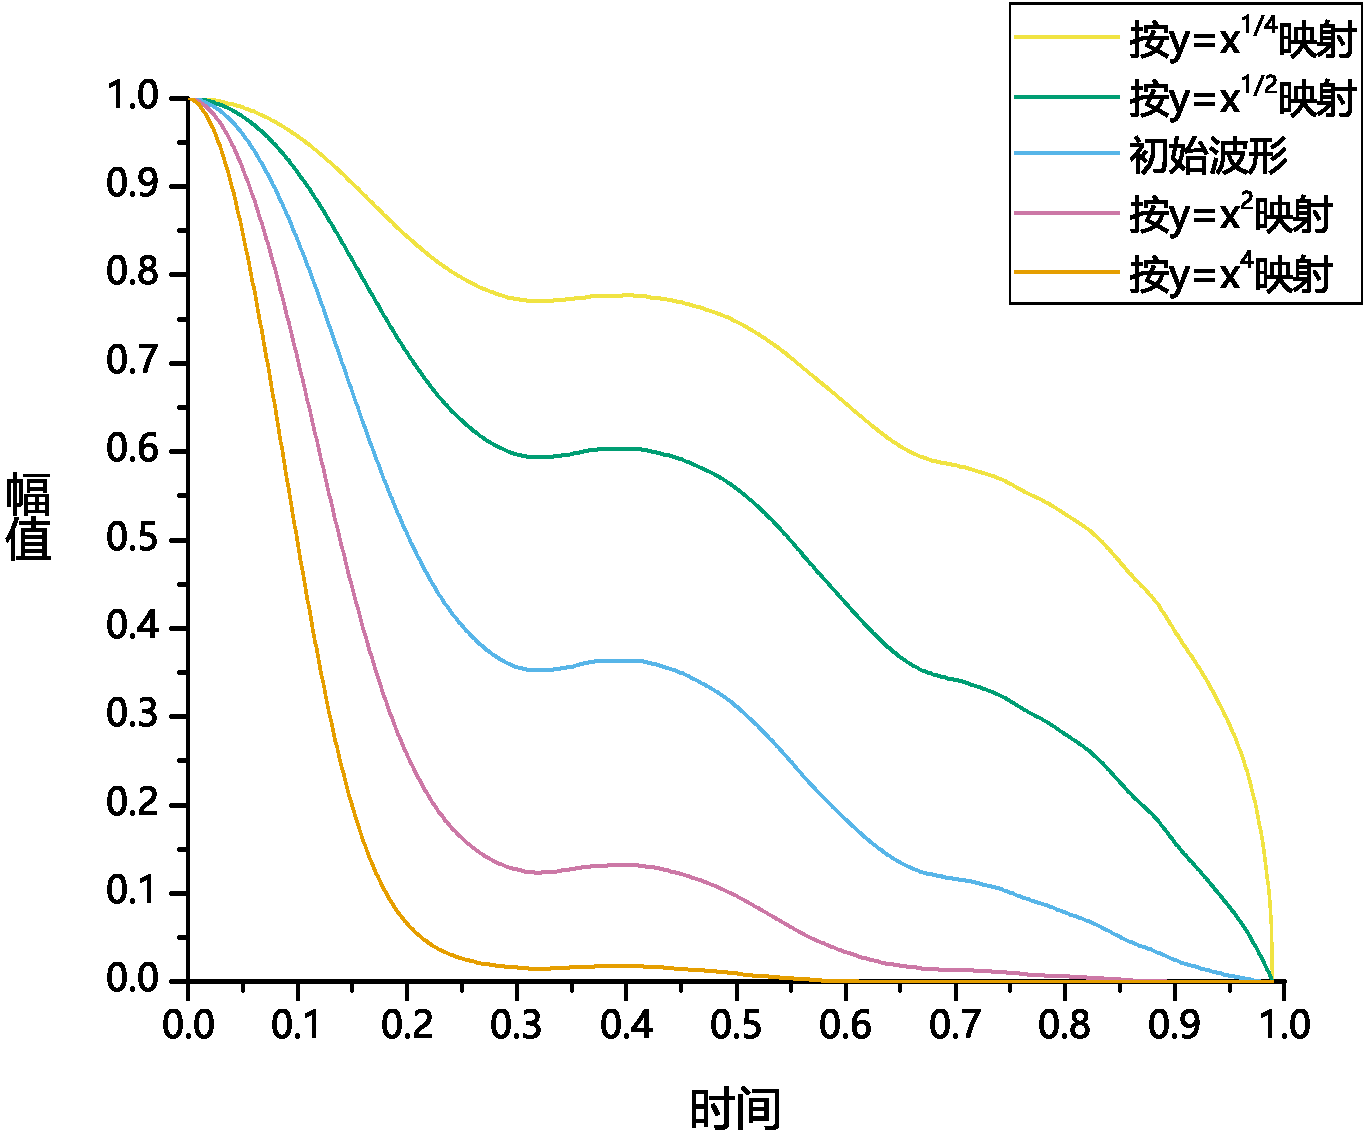
\includegraphics[width=5.5cm]{pulse_preprocess/edi2}
    }
    \quad
    \subfigure[\label{fig:edi3}对\autoref{fig:pulsecontrast}中脉搏波波形进行EDI计算 III]{
    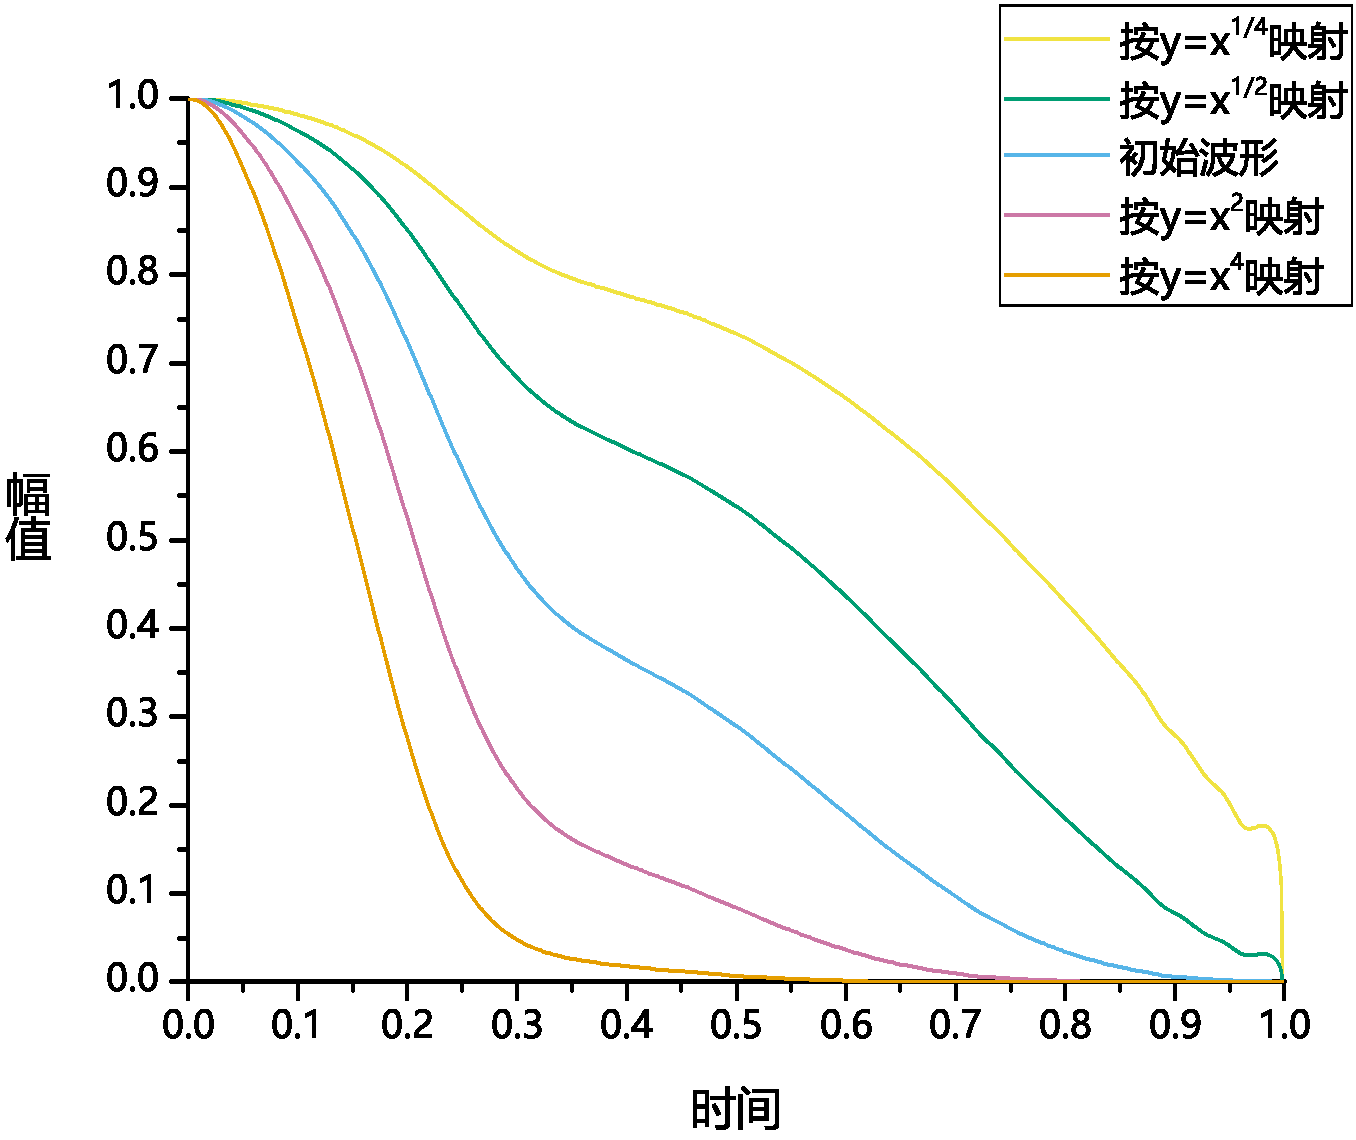
\includegraphics[width=5.5cm]{pulse_preprocess/edi3}
    }
    \caption{\label{fig:powandedi}幂函数簇与PPG波形的EDI指标示意}
\end{figure}

为解决上述问题,本研究首创提出了膨胀-腐蚀面积指数(erode and dilate area index,EDAI)这一新的描述方法。如\autoref{fig:powandedi}所示,EDAI的基本思路是利用幂函数簇的相关性质,
对\autoref{equ:area1}的累加值进行一定的映射,先对原始波形数据进行一次非线性变换
\begin{equation}
    \label{equ:area3}
    S \approx \frac{\Delta t}{2} \sum_{i=0}^{n-1}{(\boldsymbol F (P(i))+\boldsymbol F (P(i+1)))}
\end{equation}
其中,$\boldsymbol F$是幂指数函数簇。若将波形数据经幂函数$\boldsymbol F(x)=x^n$映射后的图形面积记为$S_n$,
那么,EDAI可以记为
\begin{equation}
    \label{equ:edai}
    EDAI_{k}=[S_{n_1},S_{n_2},\cdots,S_{n_k}]
\end{equation}
其中,$S_{n_k} \neq 0$。对比\autoref{equ:featurevector}可以发现,EDAI也是本研究先前定义的脉搏波波形特征描述向量的一个具体实例。

由相关数学知识可知,幂函数$\boldsymbol F(x)=x^n$在其定义域内均保持单调递增的性质。特别地,若限定函数定义域$x\subseteq [0,1]$,对于$n>1$的幂指数函数,$f(x)$均在$y=x$图像的下方,且$n$值越大,图像越贴近$x$轴,
函数图像“腐蚀”得越发严重;反之,$0<n<1$的幂指数函数会使$y=x$的图像趋近于直线$x=1$,$n$值越大,函数图像“膨胀”得愈益明显,如图\autoref{fig:pow}所示。
此时,若选取某一具体的幂函数,对所有采样点数值进行映射处理,相当于对原始波形图像进行了一次非线性拉伸变换。而幂函数本身的单调性可以保证这样的非线性缩放结果也是唯一的,
如图\autoref{fig:edi1}-图\autoref{fig:edi3}所示。若同时使用多个不同的幂函数进行上述处理,PPG波形上的差异必然在体现其对应的映射数值上,最终的面积累积值必然有所差异,
从而在面积类参数中保留了PPG波形细节信息。

\subsection{脉搏波波形间的描述}
在某些情景下,相较脉搏波间的共性特征而言,PPG波形间的差异(或者称之为PPG波形的紊乱程度)可能更需要被研究者们关注,如\autoref{fig:diff_in_pulse}所示。
如何评估、量化这种波形间乃至整条数据中所有波形之间的差异是本小节要阐述的重点。
\begin{figure}[htbp]
    \centering
    \subfigure[\label{dp0}正常孕妇的波形]{
    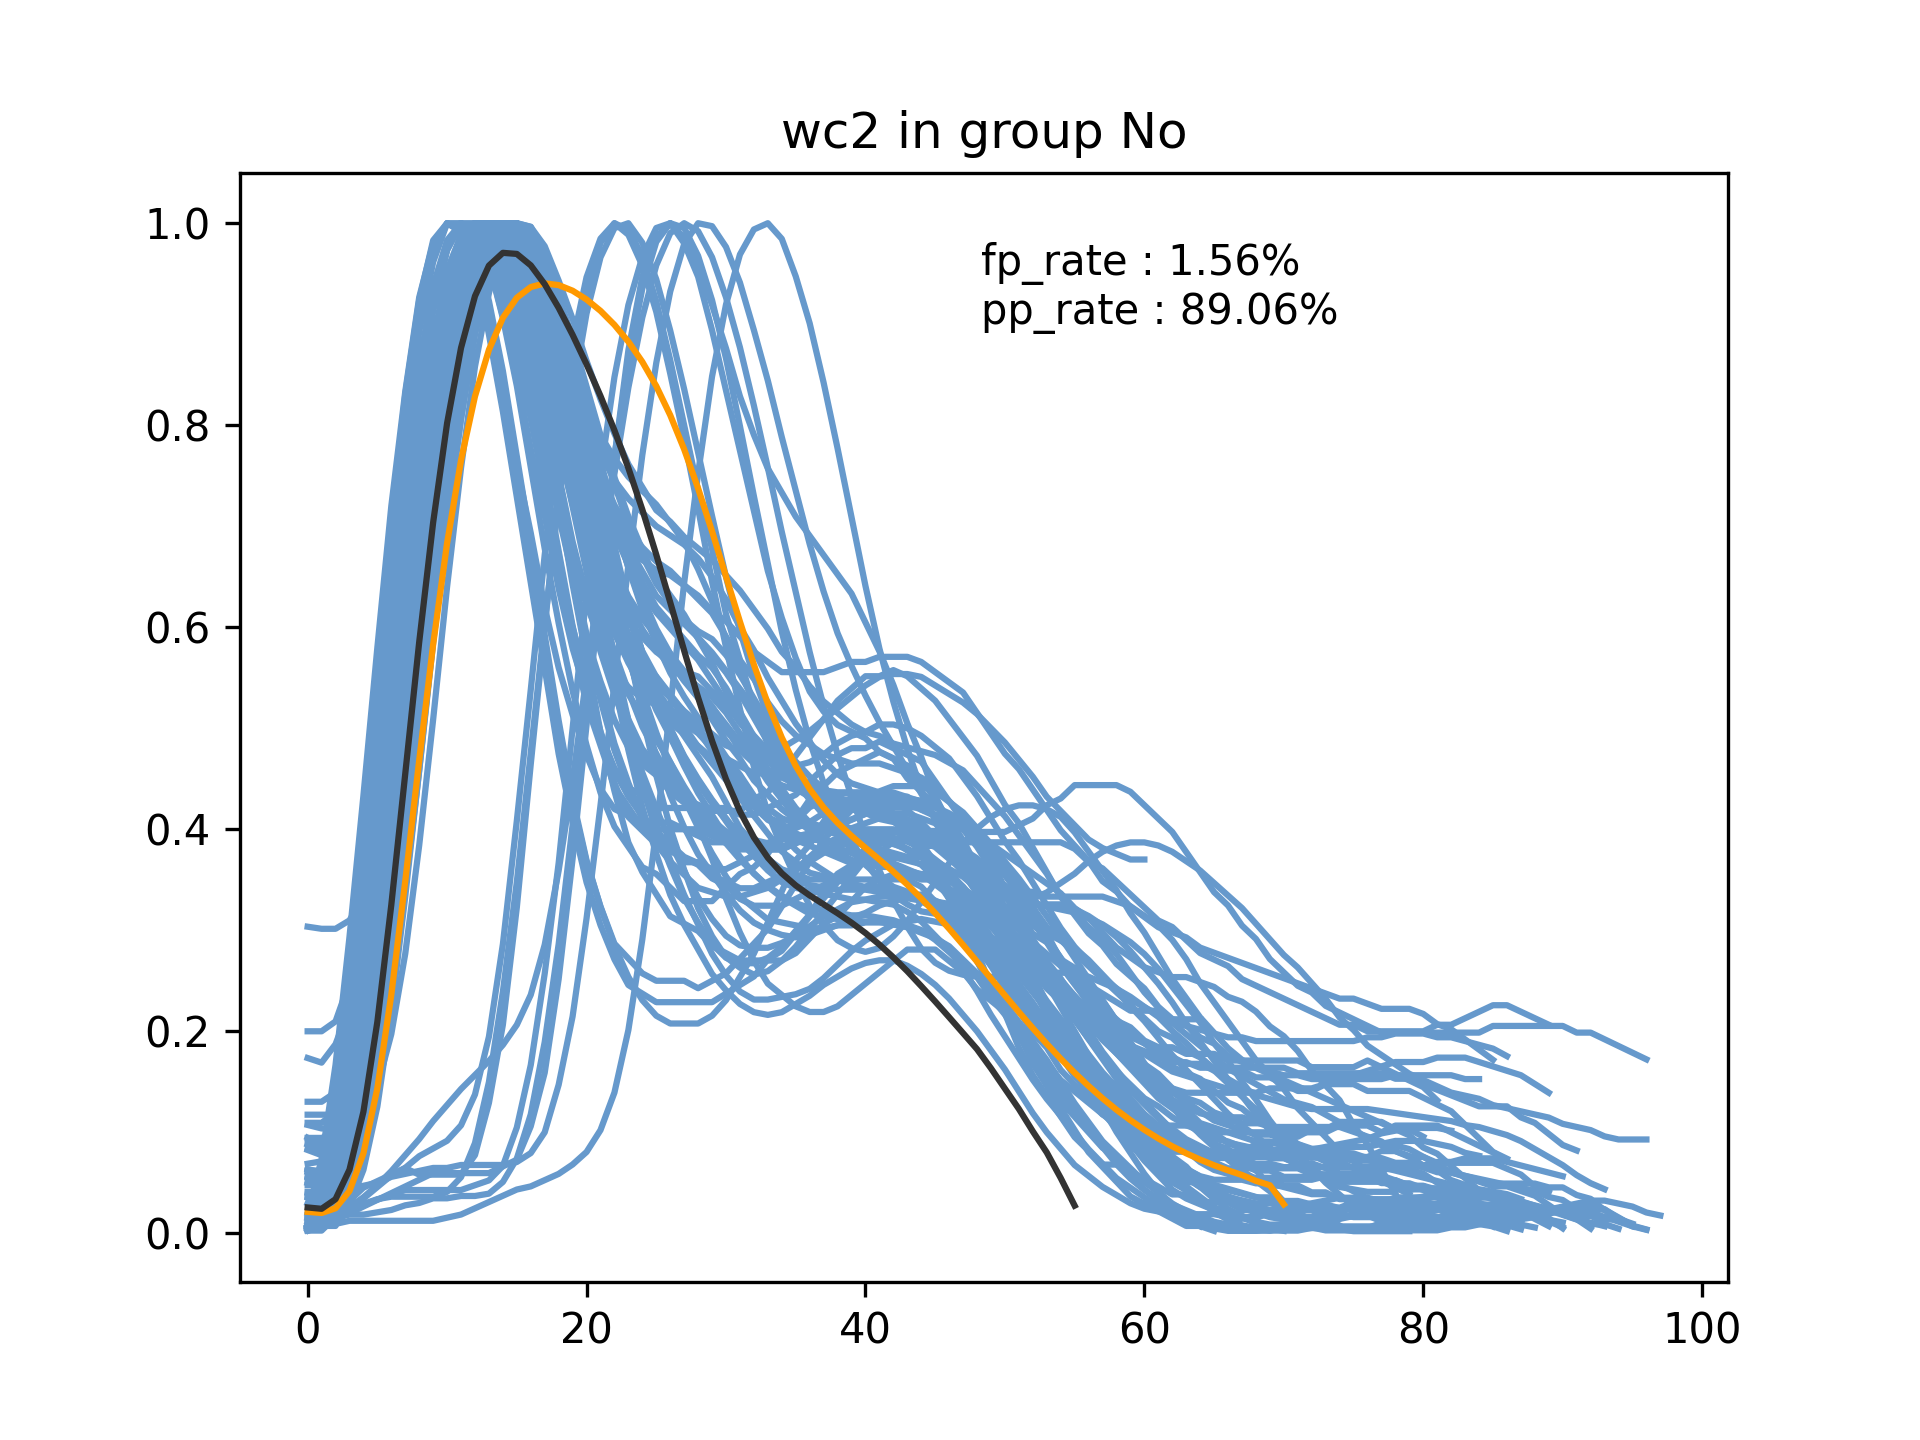
\includegraphics[width=6cm]{pulse_preprocess/wc2 in group No}
    }
    \quad
    \subfigure[\label{fig:dp1}患有PE孕妇的波形]{
    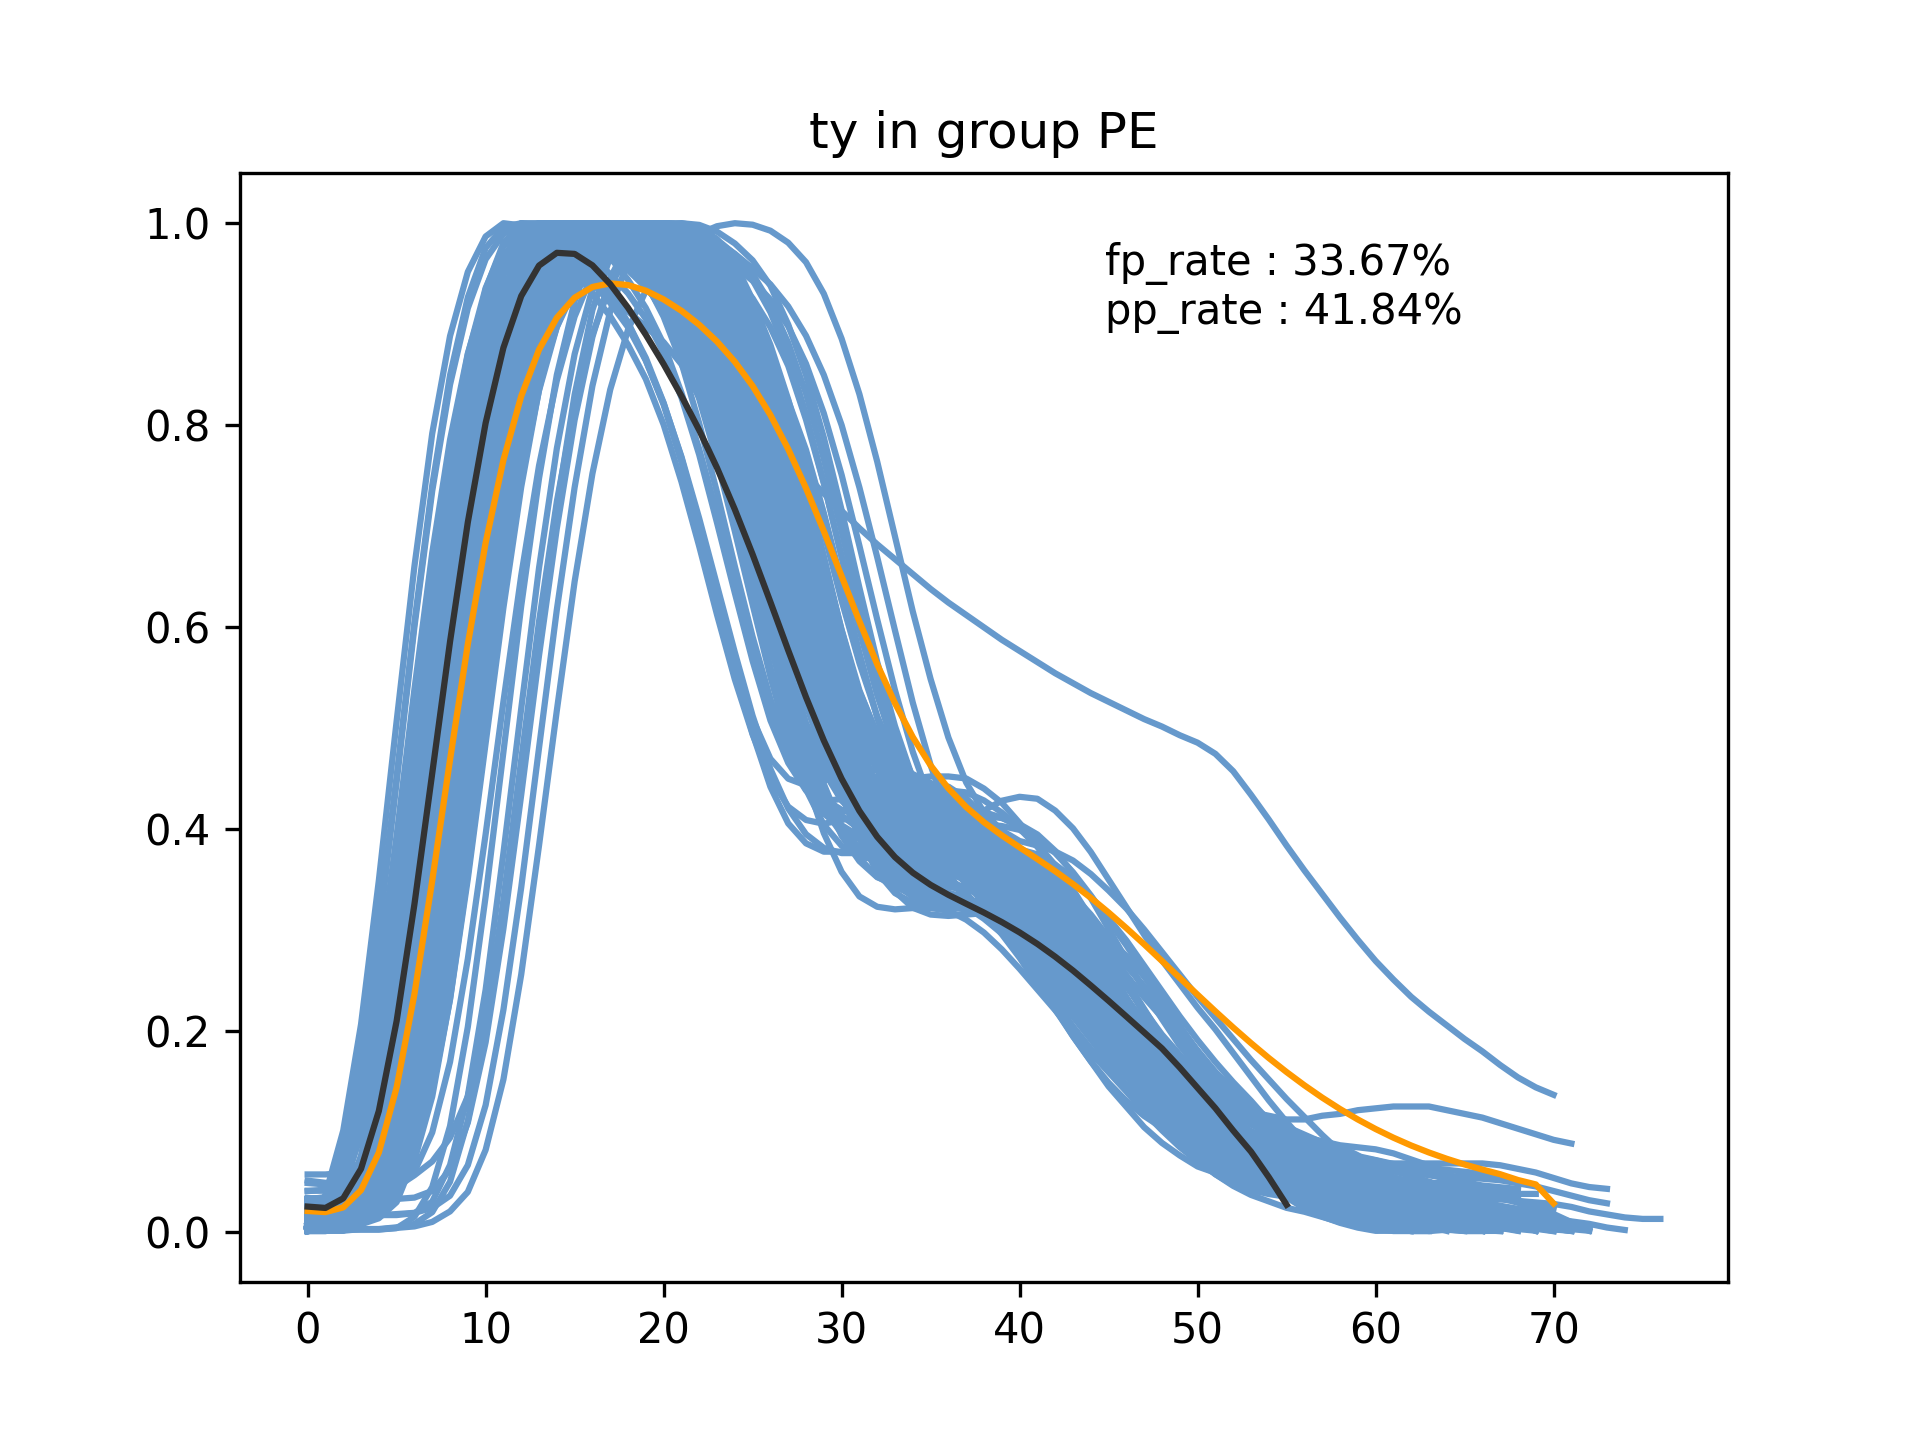
\includegraphics[width=6cm]{pulse_preprocess/ty in group PE}
    }
    \caption[脉搏波波形间的差异性]{\label{fig:diff_in_pulse}脉搏波波形间的差异性。使用了本研究自行采集的数据,所有波形经标准化后按起点进行了对齐。}
\end{figure}

本章此前介绍的PPG各项特征参数的设计逻辑多数是以一个完整波形为基本单位并对其进行量化描述,若直接用这些参数描述波形间的差异,会存在描述不够直接与描述能力有局限性等两项不足。
其中,前者是指波形间的差异能在具体参数的数值上得到体现,但差异的具体程度有待商榷;后者是指若出现涉及多个波形间的差异比较的情景,之前的参数会更显乏力。
鉴于此,本研究特进行了以下探索性研究。

一、两个波形的差异描述

本研究提出了互相关系数、Frechet距离及包络面积等三种参数量化描述脉搏波波形间的差异性。
此外,还对这三种参数的最容易遇到的对齐问题给出了一种可行解决思路。

1. 描述参数

\Rnum{1}. 相关系数

本文的第二章已经介绍过相关系数的这一变量分析方法,如\autoref{fig:relation}所示。由于相关系数本身就是作为衡量两个变量因素的密切程度而设计的,
因此,一种可行的办法是直接用相关系数去衡量两个波形之间的“相似”程度。需要注意的是,斯皮尔曼相关系数在计算时要求必须原始数据进行排序操作,而这一操作无疑会直接破坏波形的数据信息。
故本文最终选取了皮尔逊相关系数$r_p$进行表征
\begin{equation}
    \label{equ:pearson2}
    r_p=\frac{\sum_{i=1}^n{(x_i- \mathop{x} \limits^-)(y_i- \mathop{y} \limits^-)}}{\sqrt{{\sum_{i=1}^n}{{(x_i- \mathop{x} \limits^-)^2\sum_{i=1}^n}{(y_i- \mathop{y} \limits^-)^2}}}}
\end{equation}
波形间相关系数值越大,两者越“相似”。

\Rnum{2}. 弗朗明歇距离

弗朗明歇距离(Fréchet distance,FD)是最早由法国数学家Maurice René Fréchet于1906年提出的一种路径空间相似形描述方法\cite{Wien1994,Kaveh2013,GN2017}。
\autoref{fig:frechet distance}给出了FD定义的示意图。一种最经典、形象的理解是人牵着一条狗沿着不同的轨迹行走,两者之间最大的最短距离就是狗绳长度的下限,
这个值即为弗朗明歇距离。
\begin{figure}[htbp]
    \centering
    \subfigure[\label{fd0}弗朗明歇距离的形象示意]{
    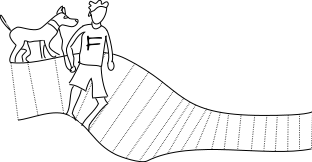
\includegraphics[width=6cm]{pulse_preprocess/frechet_distance0}
    }
    \quad
    \subfigure[\label{fig:fd1}弗朗明歇距离的数学示意\cite{GN2017}]{
    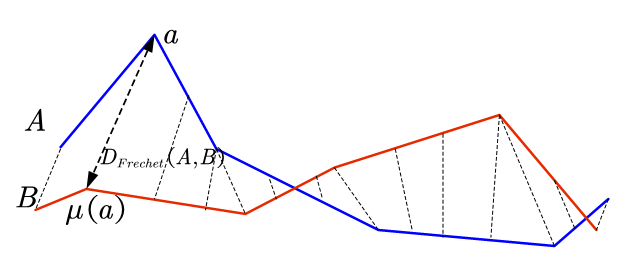
\includegraphics[width=6cm]{pulse_preprocess/frechet_distance1}
    }
    \caption{\label{fig:frechet distance}弗朗明歇距离的定义}
\end{figure}

FD的完整数学定义如下,若将曲线视为其在定义域至度量空间的一种映射关系,即$[a,b]\rightarrow V$,
那么对曲线$f:[a,b]\rightarrow V$与曲线$g:[a',b']\rightarrow V$,两者的弗朗明歇距离为
\begin{equation}
    \label{equ:frechet distance}
    \delta_F(f,g)=\inf \max \limits_{\alpha,\beta \; t \in (0,1)} d(f(\alpha(t)), g(\beta(t)))
\end{equation}
其中,$\alpha$与$\beta$是满足能将$[0,1]$分别映射至$[a,b]$与$[a',b']$的任意连续非递减函数,$d$是$V$上的度量函数\cite{Wien1994}。
一般而言,弗朗明歇距离的计算是个递归过程。
波形间的弗朗明歇距离值越小,两者越“相似”。

\Rnum{3}. 包络面积差

包络面积差(difference of envelope area ,DEA)是本研究提出的用以描述脉搏波间差异的原创指标。如\autoref{fig:dea}所示,其计算原理是计算两个经幅值归一化后的波形的按起点对齐后,由这两个波形围起来的区域的累计面积
\begin{equation}
    \label{equ:dea}
    \begin{aligned}
        S &= \int_{t_0}^{t_n}|P_f(t)-P_g(t)|dt\\
        &\approx \frac{\Delta t}{2} \sum_{i=0}^{n-1}{|(P_f(i)+P_f(i+1)-(P_g(i)+P_g(i+1))|}
    \end{aligned}
\end{equation}
\begin{figure}[htbp]
    \centering
    \subfigure[\label{fig:dea0}原始采样的包络面积差示意]{
    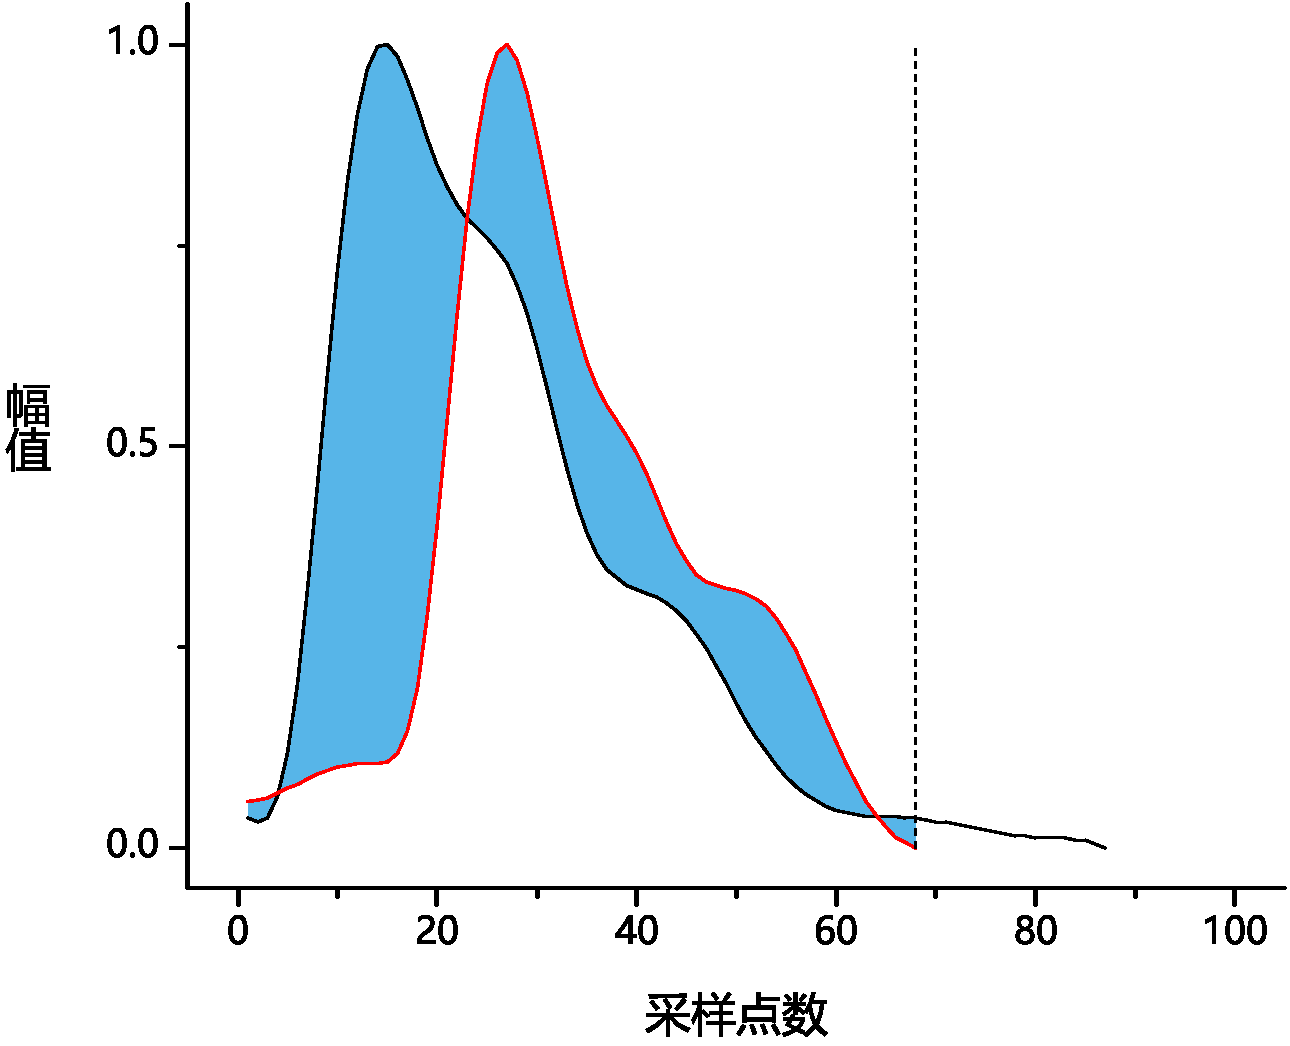
\includegraphics[width=6cm]{pulse_preprocess/dea0}
    }
    \quad
    \subfigure[\label{fig:dea1}重采样后的包络面积差示意]{
    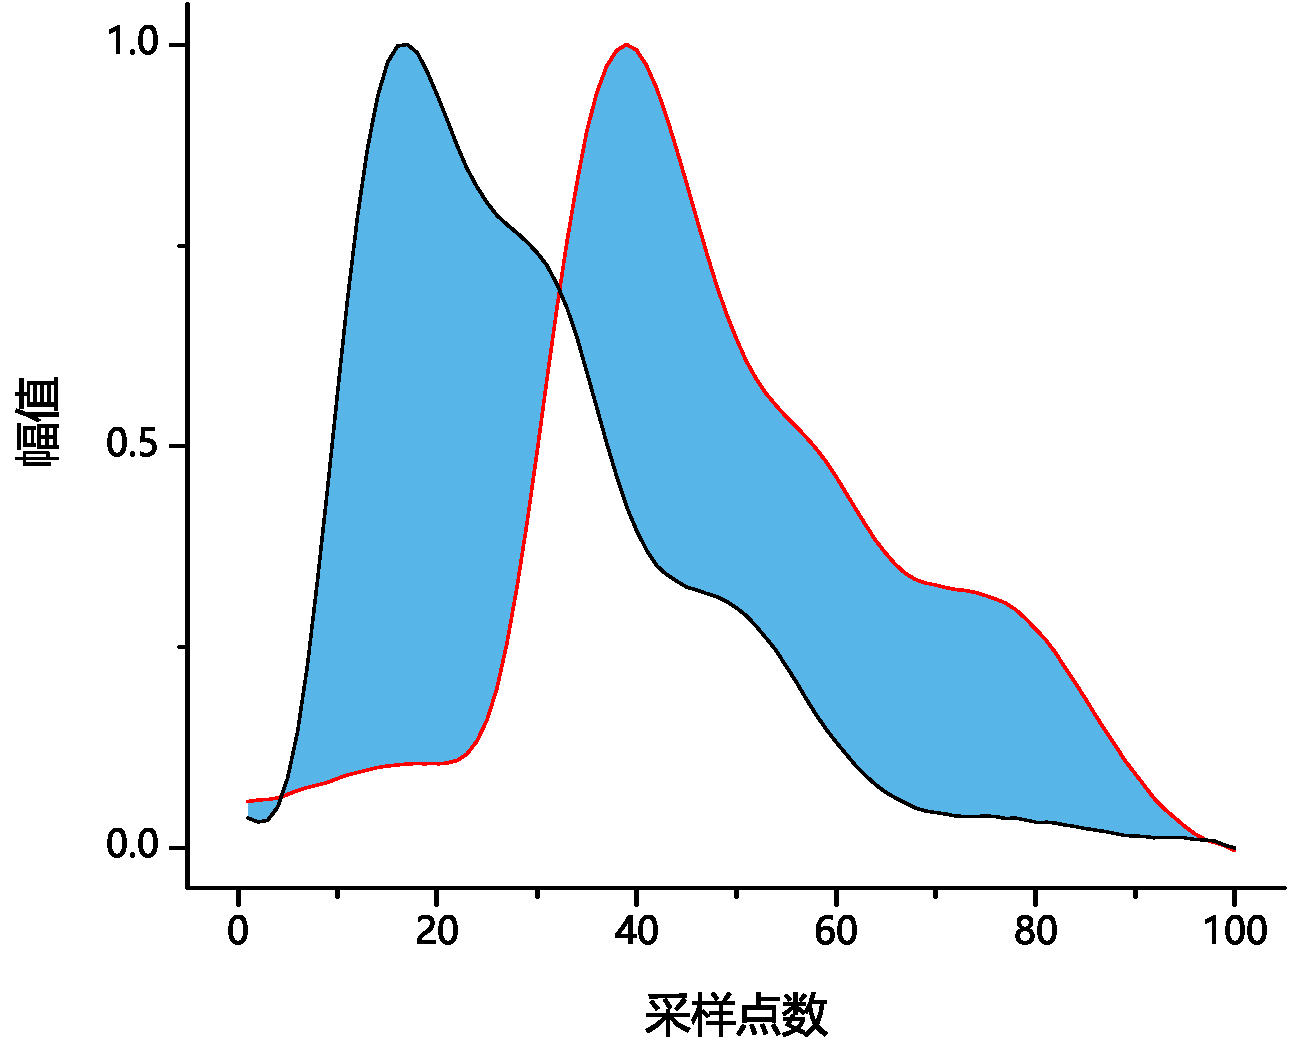
\includegraphics[width=6cm]{pulse_preprocess/dea1}
    }
    \caption[包络面积差示意]{\label{fig:dea}包络面积差示意。注意左图中虚线之后的数据处理。}
\end{figure}
波形间包络面积差值越小,两者越“相似”。

2. 波形采样点对齐

上述三个描述参数的计算过程都包含了一个隐藏的前置条件,即参与计算的两个波形的时间序列有着相等的采样点数。但如\autoref{fig:diff_in_pulse}与\autoref{fig:dea}所示,
由于脉搏波信号本身的随机性,这样的条件在实际中几乎不可能被满足。这也要求我们在计算这些参数时必须考虑波形的采样点数对齐问题。若将参与比较的两个波形的采样点数
分别记为$m$、$n$且$m \neq n$,不失一般性,设$m>n$,那么可行的解决思路有以下三种:

\Rnum{1}. 长端截取

此思路是只对两波形的前n个采样点进行计算,较长波形剩余$m-n$个采样点不参与计算。

\Rnum{2}. 短端补值

此思路是对较段波形在末端进行补值处理使其采样点数也为$m$,新增的补值可以设为0。

\Rnum{3}. 重采样至相同数值

与上述的截取、补值处理不同,重采样的处理逻辑是将两个波形的采样点数调整至相同。如在本章信号预处理小节中介绍的,通过信号的插值与抽取即可调整数据采样率。
若需将采样长度为$m$的波形调整至$k$,记$m$与$k$的最小公倍数为$p$,此时只需将原始数据均匀插值至$p$点,再按每$p/k$个点进行抽取即可。重采样前后的波形对比如\autoref{fig:dea}所示。

最后,需要指出的是,弗朗明歇距离的计算过程是一个递归过程,目前很多具体的实现算法均已可以对长度不对齐的两个序列进行计算\cite{derohde2022}。

二、更多波形间的差异性描述

前文介绍的是对两个波形间的差异的描述,对更多的波形间的描述也可按照这种思路进行。具体而言,若需量化\autoref{fig:diff_in_pulse}所示n个波形间的整体差异性,可按排列组合的方法每次从n个波形间
选取两个波形,并用上述三种描述参数进行量化,最终会得到3组数据,每组有$C_n^2$个具体数值。此时,可按数理统计的一般方法,用这3组数据的平均值、方差、标准差、极值等指标进行这n个
波形的整体性描述。

\section{脉搏波时域特征集的构建}
作为构建能够识别PE的ML模型的数据准备,本章在第三章介绍过的PPG波形的新型时域特征的设计基础上,确定了这些新型参数的具体计算标准与方法。得到的基于时长、角度、斜率与面积等维度的新型特征构成了
\textbf{脉搏波多维度时域特征集}(photoplethysmographic multidimensional time-domain feature set,PPGMTFS)。
本章也将PPG的原始采样值视为一种特殊的描述特征,将一个完整的PPG波形的全部采样值视为\textbf{脉搏波采样值时域特征集}(photoplethysmographic sample-value-based time-domain feature set,PPGSTFS)。
由于设计理念不同,本论文并未将以上两个特征集进行合并或交叉处理,这两个特征集合各自被\textbf{独立地}用作后续PE识别分析阶段的输入数据。

\subsection{脉搏波多维度时域特征集}

依据第三章中PPG波形的新型时域特征的设计基础,只要在PPG波形上的确定任意点$Q$,都可以得到与之唯一关联的一系列基于线段、曲线长度、斜率、弧度及面积等多维度时域特征,如\autoref{fig:point}所示。
从采样的角度而言,当选取了足够多的这样的基准参考点,就可以用与这些基准点关联的多维度时域特征描述PPG波形。此时,这些多维度时域特征也必然是以向量的形式存在的,
也即第三章介绍过的脉搏波特征描述向量(photoplethysmographic feature vector,PPGFV)。

\begin{figure}[htbp]
  \centering
  \subfigure[\label{fig:lv}左视类指标示意]{
  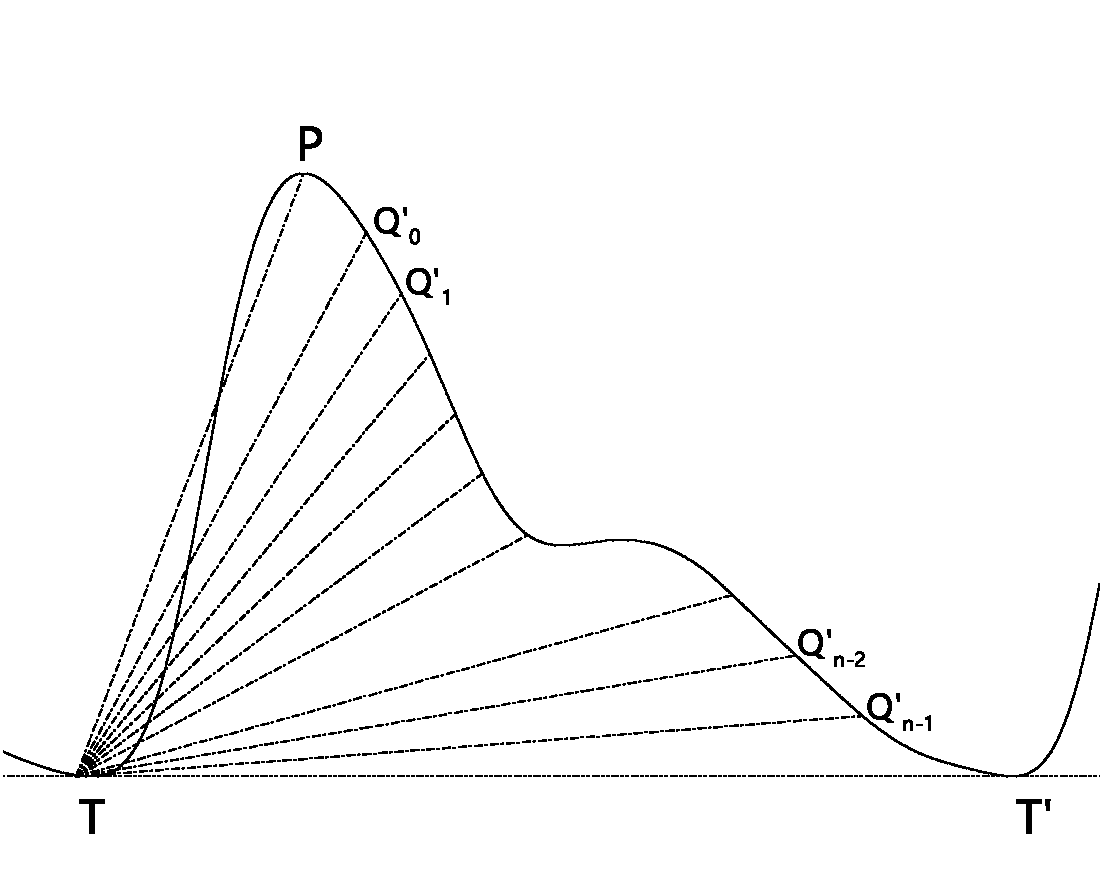
\includegraphics[width=6.5cm]{features/lv}
  }
  \quad
  \subfigure[\label{fig:cv}中视类指标示意]{
  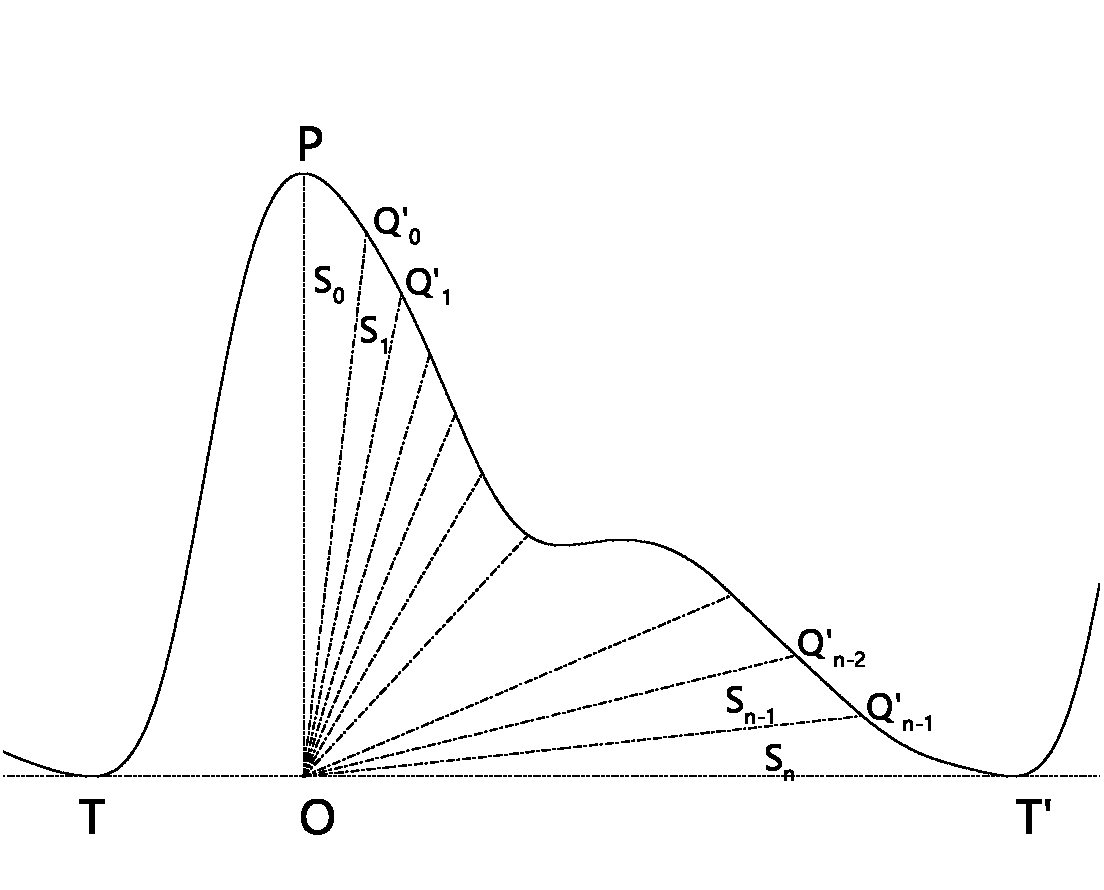
\includegraphics[width=6.5cm]{features/cv}
  }
  \quad
  \subfigure[\label{fig:sv}分层类指标示意]{
  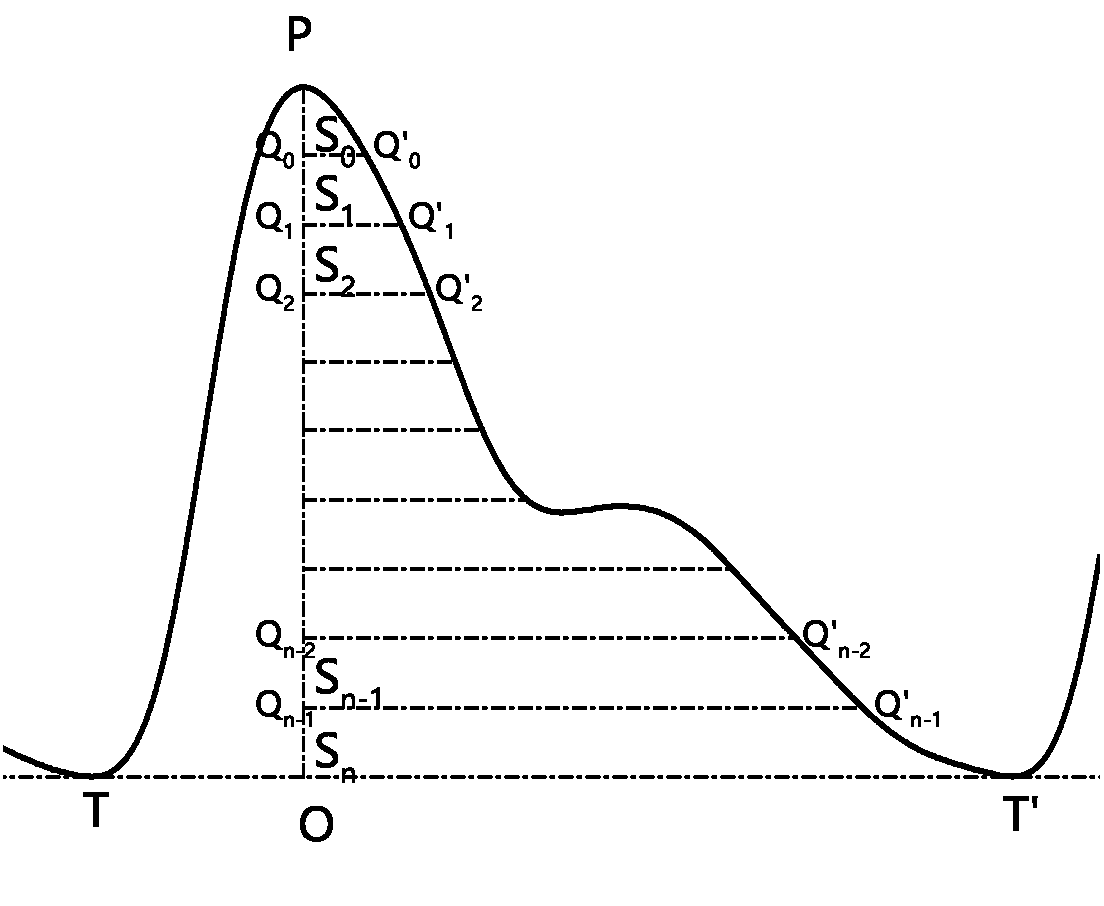
\includegraphics[width=6.5cm]{features/sv}
  }
  \caption{\label{fig:all_views}确定基准点的三种策略示意}
\end{figure}

在PPG波形上选取并确定基准点的过程,是通过PPGFV对PPG进行描述的关键。
根据选取基准点的方式,本研究共使用了三种策略,分别为左视策略(left view strategy,LVS)、中视策略(center view strategy,CVS)与分层策略(scaled view strategy,SVS)。
这三种策略的概念图如\autoref{fig:all_views}所示。

一、LVS

LVS以PPG上升支起点为原点$T$,同时将PPG波峰设为$P$,将线段$TP$与水平基线$TT'$所构成的夹角$\angle PTT'$等分成若干份。这些等分线与PPG的交点${Q'}_i$被确定为参考基准点,这一过程如图\autoref{fig:lv}所示。

二、CVS

CVS以PPG波峰$P$在水平线$TT'$上的映射点$O$为中心,将线段$OP$与水平基线构成的两个夹角$\angle POT$与$\angle POT'$等分成若干份。将这些等分线与PPG的上升支、下降支的交点计为参考基准点${Q'}_i$,这一过程如图\autoref{fig:cv}所示。

三、SVS

SVS将PPG波峰$P$在水平线$TT'$上的映射点计为$O$,作线段$OP$的水平垂线将$OP$等分为若干份。将这些等分线与PPG的上升支、下降支的交点计为参考基准点${Q'}_i$,这一过程如图\autoref{fig:sv}所示。

基准点的维数在本研究中也被统一设置为10,该值是在完整描述PPG的前提下避免出现信息冗余的折中选项。
经由这些策略得到的基准点最终确定得到的多维度时域特征如\autoref{tab:allfeatures}所示。
在计算这些特征的具体数值前,PPG波形全部进行了标准化设置,波形幅值被调整缩放至[0,1000]区间内,其中PPG波形的上升支与下降支分别按第三章的介绍过的线性变换思想进行了处理。
该标准化过程中涉及的斜率与截距参数也在\autoref{tab:allfeatures}进行了补充。

\begin{center}
  \zihao{5}
  \begin{longtable}{m{1.5cm}<{\centering}m{3.5cm}<{\centering}m{2cm}<{\centering}m{8cm}<{\centering}}
    \caption{由三种策略确定的PPG多维度时域特征集合}\\
    \label{tab:allfeatures}\\
        \topline
        \colorhead \textbf{类别}&\textbf{特征名称}&\textbf{缩写符号}&\textbf{物理意义}\\
        \midline
        \endfirsthead
        \caption[]{(续)}\\
        \midline
        \colorhead \textbf{类别}&\textbf{特征名称}&\textbf{缩写符号}&\textbf{物理意义}\\
        \midline
        \endhead 
        \midline
        \endfoot
        \bottomline
        \endlastfoot
        \colorrowa &     左视斜率    &   LVS    &   各等分线所对应的直线斜率   \\
        \colorrowa &     左视上升支交点坐标 & LVLR & 等分线与PPG波形上升支交点横坐标 \\
        \colorrowa &     左视下降支交点坐标 & LVLF & 等分线与PPG波形下降支交点横坐标 \\
        \colorrowa \multirow{-4}*{左视策略}&     左视上升支交点距离 & LVRR & 等分线与PPG波形上升支交点与波形起点距离 \\
        \colorrowa &     左视下降支交点距离 & LVRF & 等分线与PPG波形下降支交点与波形起点距离 \\
        \colorrowa &     左视交点坐标差 & LVD & 左视上升支交点坐标与左视下降支交点坐标之差 \\
        \colorrowa &     左视上升支弧长 & LVALR & PPG波形上升支被等分线分割的各区间弧长 \\
        \colorrowa \multirow{-4}*{左视策略} & 左视下降支弧长 & LVALF & PPG波形下降支被等分线分割的各区间弧长 \\
        \colorrowc &     中视上升支交点坐标 & CVLR & 等分线与PPG波形上升支交点横坐标 \\
        \colorrowc &     中视下降支交点坐标 & CVLF & 等分线与PPG波形下降支交点横坐标 \\
        \colorrowc &     中视上升支交点距离 & CVRR & 等分线与PPG波形上升支交点与峰值水平映射点距离 \\
        \colorrowc &     中视下降支交点距离 & CVRF & 等分线与PPG波形下降支交点与峰值水平映射点距离 \\
        \colorrowc &     中视交点坐标差 & CVD & 中视上升支交点坐标与中视下降支交点坐标之差 \\
        \colorrowc &     中视上升支弧长 & CVALR & PPG波形上升支被等分线分割的各区间弧长 \\
        \colorrowc &     中视下降支弧长 & CVALF & PPG波形下降支被等分线分割的各区间弧长 \\
        \colorrowc &     中视上升支面积 & CVAR & PPG波形上升支被等分线分割的各区域面积 \\
        \colorrowc \multirow{-12}*{中视策略} &     中视下降支面积 & CVAF & PPG波形下降支被等分线分割的各区域面积 \\
        \colorrowa &     分层上升支交点坐标 & SVLR & 等分线与PPG波形上升支交点横坐标 \\
        \colorrowa &     分层下降支交点坐标 & SVLF & 等分线与PPG波形下降支交点横坐标 \\
        \colorrowa &     分层上升支面积 & SVAR & PPG波形上升支被等分线分割的各区域面积 \\
        \colorrowa &     分层下降支面积 & SVAF & PPG波形下降支被等分线分割的各区域面积 \\
        \colorrowa &     分层面积 & SVAT & PPG波形整体被等分线分割的各区域面积 \\
        \colorrowa &     分层上升支交点距离 & SVRR & 等分线与PPG波形上升支交点与峰值水平映射点距离 \\
        \colorrowa &     分层下降支交点距离 & SVRF & 等分线与PPG波形下降支交点与峰值水平映射点距离 \\
        \colorrowa &     分层交点坐标差 & SVD &  分层上升支交点坐标与分层下降支交点坐标之差\\
        \colorrowa &     分层上升支弧长 & SVALR & PPG波形上升支被等分线分割的各区间弧长 \\
        \colorrowa &     分层下降支弧长 & SVALF & PPG波形下降支被等分线分割的各区间弧长 \\
        \colorrowa \multirow{-11}*{分层策略} &     分层上升支斜率 & SVSR & 等分线与PPG波形上升支交点与PPG峰值水平映射点所形成直线的斜率\\
        \colorrowa \multirow{-1}*{分层策略} & 分层下降支斜率 & SVSF & 等分线与PPG波形下降支交点与PPG峰值水平映射点所形成直线的斜率 \\
        \colorrowc &     上升支标准化斜率 & STDKR & 标准化PPG上升支波形至[0-1000]时使用的斜率 \\
        \colorrowc &     上升支标准化截距 & STDBR & 标准化PPG上升支波形至[0-1000]时使用的截距 \\
        \colorrowc &     下降支标准化斜率& STDKF & 标准化PPG下降支波形至[0-1000]时使用的斜率 \\
        \colorrowc \multirow{-4}*{标准化指标}   &  下降支支标准化截距 & STDBF & 标准化PPG上升支波形至[0-1000]时使用的截距 \\
  \end{longtable}
\end{center}
\vspace{-1.2cm} 
\subsection{脉搏波采样值时域特征集}

前文中介绍的所有PPG特征均是在原始采样值的基础上,经一定的数学处理后,间接对PPG波形进行描述的。由于PPG信号的原始采样值本身就是一种量化描述,
故本文将其作为一种特殊的直接描述PPG波形的特征。
从这个角度而言,一个完整波形的所有采样值可视为向量维数即为采样数的特殊PPGFV。

\autoref{fig:no_pe}对比展示了四例被试的PPG波形的采样值差异,其中,各子图在同一坐标系下绘制了同一被试的所有PPG波形,这些波形均按起点进行了对齐,波形的采样值经标准化后被调整至[0,1]区间。

\begin{figure}[htbp]
  \centering
  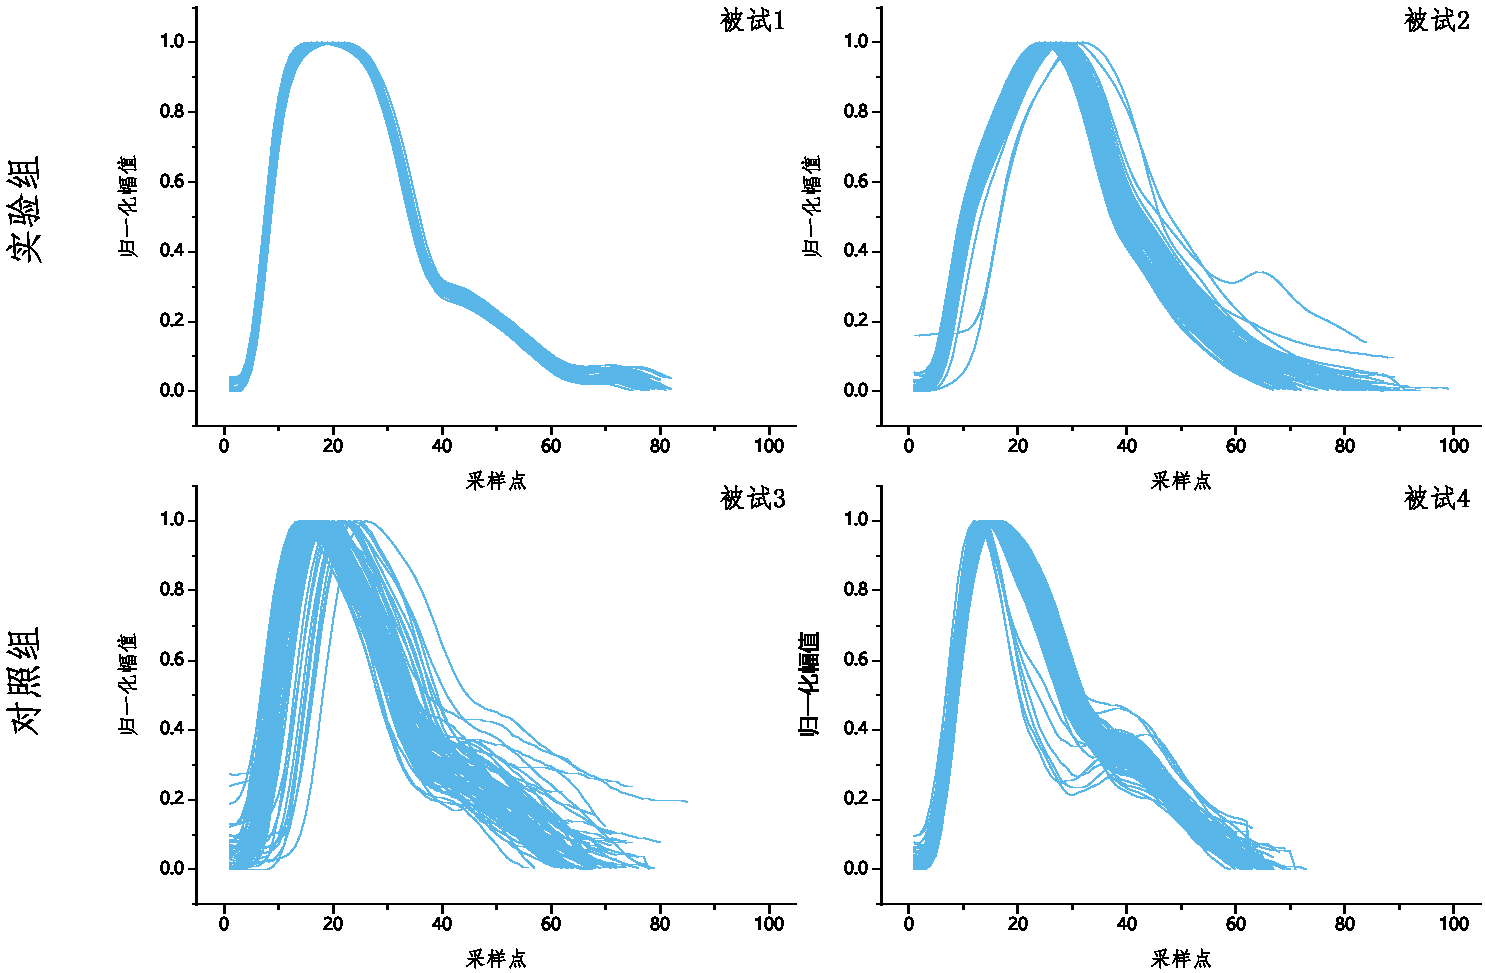
\includegraphics[width=0.75\linewidth]{features/ppgs}
  \caption{\label{fig:no_pe}被试孕妇PPG经标准化处理后的波形对照}
\end{figure}

从\autoref{fig:no_pe}可以看到,实验组与对照组的被试在PPG波形形态及整体分布上均呈现出一定的差异,这说明通过采样值描述PPG波形的可行性。
此外,从\autoref{fig:no_pe}也可以看到,即使对同一被试而言,不同PPG波形之间也存在这较为明显的时长差异。若不加任何处理,这种差异会直接导致PPGSTFS的维数差异。
为消除这种维数差异可能带来的影响,本文提出了三种处理策略进行PPG波形对齐操作,分别为重采样策略(resampling strategy, RS)、补齐策略(complementary strategies,CS)
与截取策略(interception strategy,IS)。为说明三种策略处理思路,下面以两个PPG波形的对齐处理过程为例,记这两个波形的原始采样数分别记为$m$、$n$且$m \neq n$,不失一般性,设$m>n$。

一、RS

RS主要通过信号的插值与抽取调整数据采样率,随后将两个PPG波形的采样点数调整至相同数值$n_r$。
若按RS将采样长度为$m$的波形调整至$n_r$,记$m$与$n_r$的最小公倍数为$p$,只需将原始数据均匀插值至$p$点,再按每$p/n_r$个点进行抽取即可。

由于采集得到的绝大多数PPG波形采样点数不足80,本研究最终将$n_r$值设置为100。
该值保证了PPG波形的描述的分辨率与精度,同时可保证只有极少数波形需要进行采样点的压缩。
将\autoref{fig:no_pe}中的被试数据进行重采样处理,所得的最终结果如\autoref{fig:no_pe2}展示。

\begin{figure}[htbp]
  \centering
  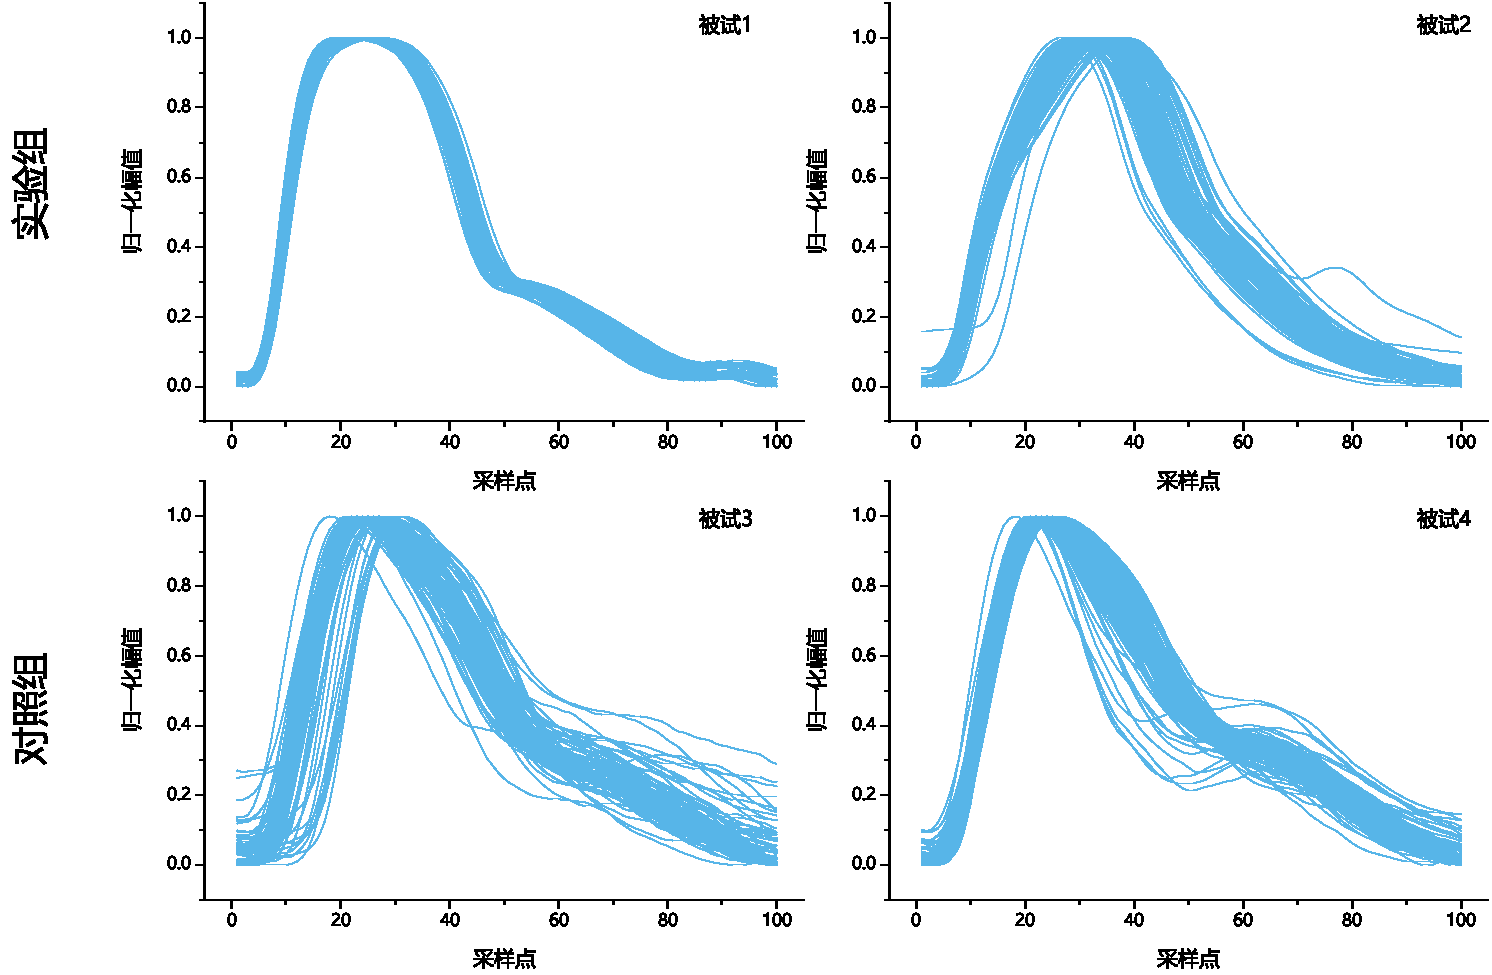
\includegraphics[width=0.75\linewidth]{features/ppgs1}
  \caption{\label{fig:no_pe2}被试孕妇PPG经标准化、重采样处理后的波形对照}
\end{figure}

二、CS

CS则是以采样点数为$m$的PPG波形为基准,对两一个波形在尾端直接进行补零处理,使两者的采样点均达到$n_c$($n_c=m$)。

由于本文得到的实验数据采样率为100$Hz$,$n_c$值被设为120。与这一数值对应的PPG波形周期也高达1.2$s$,该值已经超过了本研究采集得到的任一有效的PPG波形周期。

三、IS

与CS相反,IS会以采样点数为$n$的PPG波形为基准,舍弃掉另一个波形在$n$点以后的采样值,使两者的采样点均达到$n_i$($n_i=n$)。此过程不可避免地出现了数据损失,故这种策略被暂时弃用。

\section{脉搏波时域特征集的处理}
数据是为具体的ML研究问题而准备的,故在对数据进行下一步处理前,有必要明确本文需要研究的具体ML的问题与任务。本小节对本文要开展的具体ML研究问题进行了介绍。在此基础上,
为保证后续章节ML相关研究可顺利开展,对PPGMTFS与PPGSTFS等两个数据集的预处理工作进行了说明。此部分工作主要包括数据集的划分、特征缩放及特征降维等。

\subsection{关于子痫前期的猜想与具体机器学习方向}
绪论中已经阐述过,本文的研究目标是探寻通过PPG识别判断PE病发的可能,而该目标本质上可以划分为ML领域内的二分类任务。
而本文对PPG与PE之间的可能潜在的关系,提出了以下两种猜想。

一、\textbf{单个PPG波形可以反映PE的病发状态}

这种猜想认为PPG的波形是孕妇PE病发状态的稳定“表达”,单个PPG波形包含了可以识别区分PE的全部信息。换言之,该猜想认为由PE导致的病生理变化可以在单个波形上得到全部体现,
单个PPG波形能够作为分析识别PE的最小分析对象。

二、\textbf{被试的全部PPG波形才可以反映PE病发状态}

这种猜想认为PPG的单个波形是孕妇PE病发状态的不稳定“表达”,但孕妇的一段时间内采集得到的所有PPG波形包含了可以识别区分PE的全部信息。换言之,该猜想认为由PE导致的病生理变化可以在孕妇
的多数PPG波形的形态特征上得到全部体现,需要被试的全部PPG波形进行一个类似“群体决策”的过程。

针对上述两个猜想,本研究拟从以下两个方向展开了具体研究工作:

一、基于波形的研究

基于波形的研究(pulse-based research,PR)将单个PPG波形作为分析识别PE的最小分析对象,并进行ML算法模型的研究。此研究方向下,同一被试的PPG数据可能对应ML模型训练与验证阶段的多个数据样本,这种方式相对地增加了
数据集的样本容量。

二、基于被试的研究

基于被试的研究(subject-based research,SR)将单个被试的所有PPG波形作为一个整体进行分析处理,并进行ML算法模型的研究。此研究方向下,同一被试的PPG波形只会出现在训练集或测试集之中,
测试集中的数据样本对于训练得到的模型是完全陌生的未见示例,因此更考验ML模型的泛化能力。

\subsection{数据集的划分}
数据集的划分是监督学习在开始模型训练前必不可少的重要步骤,是将原始数据集划分为训练集与测试集的过程。其中,训练集作为训练模型的输入数据,而测试集则是用来评估该模型在未见示例上的泛化能力。

第三章已经介绍过,本文共采集得到79例被试孕妇的有效PPG数据波形共计7864个,其中,实验组44名被试包含有效波形4683个,对照组35名被试包含波形3181个。
由于本文使用了PPGMTFS与PPGSTFS等两个数据集,并提出了PR与SR等两个具体研究方向,且后续章节在进行研究时也使用了多种ML算法进行模型的构建,数据集的合理划分显得尤为重要。
本文从以下方面进行了处理工作。

一、按合理比例划分

前人的研究已经证实,在进行数据划分时,测试集包含的样本数量与全部样本的比例的最优区间在[20\%, 30\%]\cite{Gholamy2018Why7O}。
本文将该划分比例数值设为20\%,即按照训练集与测试集4:1的比例分别按被试与波形对原始数据抽样。

二、分层抽样

由于本文实验得到的PPG数据在是否患有PE的这一问题上存在分布不平衡现象,直接使用纯随机方法抽样有可能导致抽样偏差,最终影响准确性、稳定性与鲁棒性等模型效果\cite{Aurélien2018}。
为了避免此情况发生,本研究额外应用了分层抽样的策略划分数据集,将数据样本按其是否属于实验组分成两组,对新得到的两组数据
分别按照4:1比例进行抽样,两组对应的抽样结果在合并之后才形成最终的训练集与测试集。

三、固化抽样结果

为使后续多种ML模型的性能具有可比行,必须保持数据集的划分在整个研究过程中的一致性。因此,前两步中的分层抽样过程只进行一次,随即被固化保存。该划分结果在之后的ML过程中不再进行任何其他调整,
供所有ML算法训练模型或进行测试使用。

最终的数据集划分结果如\autoref{tab:dataset}所示。
\begin{center}
  \zihao{-5}
  \begin{longtable}{m{1.5cm}<{\centering}m{1.5cm}<{\centering}m{1.5cm}<{\centering}m{1.5cm}<{\centering}m{1.5cm}<{\centering}m{1.5cm}<{\centering}}
    \caption{数据集划分结果}\\
    \label{tab:dataset}\\
        \topline
        \colorhead & & \multicolumn{2}{c}{\textbf{训练集}} & \multicolumn{2}{c}{\textbf{训练集}}\\
        \colorhead \multirow{-2}{*}{\textbf{研究方向}}& \multirow{-2}{*}{\textbf{研究方向}}& \textbf{实验组} & \textbf{对照组} & \textbf{实验组} & \textbf{对照组} \\
        \midline
        \endfirsthead
        \caption[]{(续)}\\
        \midline
        \colorhead & & \multicolumn{2}{c}{\textbf{训练集}} & \multicolumn{2}{c}{\textbf{训练集}}\\
        \colorhead \multirow{-2}{*}{\textbf{研究方向}}& \multirow{-2}{*}{\textbf{研究方向}}& \textbf{实验组} & \textbf{对照组} & \textbf{实验组} & \textbf{对照组} \\
        \midline
        \endhead 
        \midline
        \endfoot
        \bottomline
        \endlastfoot
        \colorrowa  PR  & 7864  & 3746 & 2545 & 937 & 636 \\
        \colorrowc  SR  & 79  & 35 & 28 & 9 & 7 \\           
  \end{longtable}
\end{center}
\vspace{-0.8cm} 

\subsection{特征缩放}
一般而言,原始数据的输入特征在数值属性出现较大的差异会导致机器学习模型的性能下降、表现欠佳\cite{Aurélien2018}。为保证这些输入特征能满足特定的机器学习算法的输入要求,通常还要对这些特征的数值分布进行一定的调整,这也就是特征缩放操作。

常见的特征缩放处理原则是同比例缩放所有属性,使用的方法有归一化与标准化等两类方法。归一化方法又称为最小-最大缩放,可将所有数据的特征属性值同比例映射至[0,1]区间内
\begin{equation}
  \label{equ:maxmin}
  z = \frac{x - x_{min}}{x_{max}-x_{min}}
\end{equation}
其中,$z$为缩放后的数据,$x$需要标准化的数据,$x_{min}$与$x_{max}$分别对应这批数据的最小值与最大值。

而标准化的过程可将所有数据的特征属性调整至符合正态分布
\begin{equation}
  \label{equ:normalization}
  z = \frac{x - \mu}{\epsilon}
\end{equation}
其中,$z$为缩放后的数据,$x$需要标准化的数据,$\mu$与$\epsilon$分别对应这批数据的平均值与样本方差。

\subsection{特征降维}
机器学习模型的训练过程花费的时间成本会随着输入特征维数的增加而成非线性增加,这也就是通常而言的维数诅咒或维数灾难。
为加快模型训练速度,一种可行的策略在构建模型时尽可能只使用“与预期结果最相关的”、“最重要的”输入特征,即按照特征的贡献度对
原始数据集进行降维处理。需要注意的是,数据降维在加速训练的同时,通常也会导致模型性能的下降。因此,一般认为特征降维是机器学习过程中的一个可选项而非必选项。

特征降维在训练模型前后均可进行。在训练模型前的特征降维处理
主要依赖于特征数据属性值的分布特性进行筛选;在模型训练完成后的特征降维主要依赖于特征属性对模型的贡献程度进行筛选。
本小节在训练机ML模型前,使用统计分析中的U检验方法,评估了PPGMTFS中各特征参数与PE的相关性,进而完成了特征筛选与降维,如\autoref{tab:utest}所示。

\begin{center}
  \zihao{-5}
  \begin{longtable}{m{2.5cm}<{\centering}m{2cm}<{\centering}m{2.5cm}<{\centering}m{2cm}<{\centering}m{2.5cm}<{\centering}m{2cm}<{\centering}}
    \caption{脉搏波时域特征集\Rnum{1}数据特征的U检验结果}\\
    \label{tab:utest}\\
        \topline
        \colorhead \textbf{特征缩写}&\textbf{p值}&\textbf{特征缩写}&\textbf{p值}&\textbf{特征缩写}&\textbf{p值}\\
        \midline
        \endfirsthead
        \caption[]{(续)}\\
        \midline
        \colorhead \textbf{特征缩写}&\textbf{p值}&\textbf{特征缩写}&\textbf{p值}&\textbf{特征缩写}&\textbf{p值}\\
        \midline
        \endhead 
        \midline
        \endfoot
        \bottomline
        \endlastfoot
        \colorrowa  LVLR\_9  &  0.004 &  CVLF\_1  & \cellcolor{pink} \textbf{0.068} &  SVRR\_2  &  0.027 \\
        \colorrowc  LVLF\_1  &  \cellcolor{pink}\textbf{0.27}  &  CVLF\_2  &  0.038 &  SVRR\_3  &  0.001 \\
        \colorrowa  LVRR\_6  &  0.002 &  CVRF\_4  & \cellcolor{pink} \textbf{0.44}  &  SVRR\_4  &  0.001 \\
        \colorrowc  LVRR\_7  &  \cellcolor{pink}\textbf{0.387} &  CVD\_1   &  \cellcolor{pink}\textbf{0.159} &  SVD\_2   &  0.009 \\
        \colorrowa  LVD\_1   &  0.022 &  CVD\_2   &  0.024 &  SVD\_3   & \cellcolor{pink} \textbf{0.65}  \\
        \colorrowc  LVD\_2   &  0.006 &  CVALF\_6 &  0.02  &  SVALR\_2 & \cellcolor{pink} \textbf{0.078} \\
        \colorrowa  LVALR\_4 &  0.013 &           &        &  SVALR\_3 &  0.001 \\
        \colorrowc  LVALR\_5 &  \cellcolor{pink}\textbf{0.063} &           &        &           &               
  \end{longtable}
\end{center}
\vspace{-0.8cm} 

\autoref{tab:utest}列举出了由U检验得到的所有$p$值$>10^{-4}$的特征参数,其中,特征缩写所对应的具体特征与\autoref{tab:allfeatures}保持一致,特征缩写后的数值表示
该特征在PPGFV中的向量下标,该数值越小表示该特征在对应的PPGFV中越接近PPG波峰。由三种策略确定的PPG多维度时域特征均存在着一定数量的在PE数值上无统计差别的特征($p$值$> 0.05$),
这部分\autoref{tab:utest}特征未参与后续模型的训练,\autoref{tab:utest}对其用粉红底色加粗字体进行了突出显示。

在模型训练后的特征筛选处理可参见下一章节相关内容。

\section{小结}
本小节在第三章工作的基础上,完成了PPGMTFS与PPGSTFS等两个数据集的构建工作,对两个特征集的在构建过程中的设计思路与处理细节也进行了详细说明。此外,本章
明确了利用PPG数据通过ML方法对PE识别这一问题进行研究的具体目标,并按ML模型构建的一般要求,对两个特征集进行了预处理工作。
此部分的工作内容为下一章节的数据分析工作打下了坚实的基础。